\PassOptionsToPackage{table,xcdraw}{xcolor}

\documentclass[sigconf,review,anonymous]{acmart}
\acmConference[ESEC/FSE 2022]{The 30th ACM Joint European Software Engineering Conference and Symposium on the Foundations of Software Engineering}{14 - 18 November, 2022}{Singapore}

%\documentclass[sigconf,review,anonymous]{acmart}
%\acmConference[ESEC/FSE 2021]{The 29th ACM Joint European Software Engineering Conference and Symposium on the Foundations of Software Engineering}{23 - 27 August, 2021}{Athens, Greece}

%\acmConference[ICSE 2022]{The 44th International Conference on Software Engineering}{May 21–29, 2022}{Pittsburgh, PA, USA}

%\documentclass[sigconf,review, anonymous]{acmart}
%\documentclass[sigconf]{acmart}

\usepackage{booktabs}   %% For formal tables:
                        %% http://ctan.org/pkg/booktabs
\usepackage{subcaption} %% For complex figures with subfigures/subcaptions
                        %% http://ctan.org/pkg/subcaption
\usepackage{array}
\usepackage{amsmath,amsfonts}
\usepackage{algorithm}
\usepackage[noend]{algpseudocode}
%\usepackage{algorithmic}
\usepackage{graphicx}
\usepackage{textcomp}
\usepackage{float}
\usepackage{listings}
\usepackage{xspace}
\usepackage{multirow}
\usepackage{amsthm}
\newtheorem{definition}{Definition}
\usepackage{balance}

\usepackage[skins]{tcolorbox}

\usepackage{xcolor,pifont}
\newcommand*\colourcheck[1]{%
	\expandafter\newcommand\csname #1check\endcsname{\textcolor{#1}{\ding{52}}}%
}
\colourcheck{blue}
\colourcheck{green}
\colourcheck{red}

\newtcolorbox{myframe}[2][]{%
  enhanced,colback=white,colframe=black,coltitle=black,
  sharp corners,
  toprule=1.0pt,
  rightrule=0.3pt,
  leftrule=0pt,
  bottomrule=0pt,
  fonttitle=\itshape\scshape\large,
  left=0pt,right=5pt,top=5pt,bottom=3pt,
  attach boxed title to top right={yshift=-0.3\baselineskip-0.4pt,xshift=-5mm},
  boxed title style={tile,size=minimal,left=0.2mm,right=0.5mm,
    colback=white,before upper=\strut},
  title=#2,#1
}

%\newcommand{\code}[1]{{\footnotesize\textsf{#1}}}

\newcommand{\tool}{\textsc{FixLocator}\xspace}

\newtheorem{Definition}{Definition}
\newtheorem{Claim}{Claim}
\newtheorem{Lemma}{Lemma}
\newtheorem{Theorem}{Theorem}

\newcolumntype{L}[1]{>{\raggedright\arraybackslash}p{#1}}
\newtheorem{observation}{Observation}
\newtheorem{property}{Property}
\newcommand{\code}[1]{{\footnotesize\texttt{#1}}}
\usepackage{amsthm}
 \definecolor{dkgreen}{rgb}{0,0.6,0}
\definecolor{gray}{rgb}{0.5,0.5,0.5}
\definecolor{mauve}{rgb}{0.58,0,0.82}
\lstset{frame=tb,
  language=Java,
  aboveskip=3mm,
  belowskip=3mm,
  showstringspaces=false,
  columns=flexible,
  basicstyle={\small\ttfamily},
  numbers=left,
  numberstyle=\tiny\color{gray},
  keywordstyle=\color{blue},
  commentstyle=\color{dkgreen},
  stringstyle=\color{mauve},
  breaklines=true,
  breakatwhitespace=true,
  tabsize=4
}



\begin{document}

%\title[{\tool}: Deep Fault Localization with Code Coverage Representation Learning]{{\tool}: Deep Fault Localization with Code Coverage Representation Learning}

\title[Fault Localization to Detect Co-Change Fixing Locations]{Fault Localization to Detect Co-Change Fixing Locations}


%%%---- AUTHORS BLOCK ------

%Yi Li:New Jersey Institute of Technology;Shaohua Wang:New Jersey
%Institute of Technology;Tien Nguyen:University of Texas at Dallas

%\author{Yi Li}
%\affiliation{
%\institution{New Jersey Inst. of Technology, USA}
%}
%\email{yl622@njit.edu}
%\author{Shaohua Wang}
%\affiliation{
%\institution{New Jersey Inst. of Technology, USA}
%}
%\email{davidsw@njit.edu}
%\author{Tien N. Nguyen}
%\affiliation{
%\institution{University of Texas at Dallas, USA}
%}
%\email{tien.n.nguyen@utdallas.edu}


%\renewcommand{\shortauthors}{Li, Wang, and Nguyen}

\setcopyright{none}

\settopmatter{printacmref=false, printfolios=false}

\renewcommand\footnotetextcopyrightpermission[1]{} % removes footnote with conference information in first column


%(1) present information sorted in a way that a CNN can "see" patterns
%discriminating between faulty and non faulty statements more easily;

%(2) identify the actual crash statement to the network;

%(3) present more information to the deep neural network in the form of
%a summary of data dependences for each statement as well as source
%embedding; and

%(4) the suspiciousness of a statement is seen taking into account
%relationships to other statement, as opposed to a statement by itself”



%\input{sections/abstract}
\begin{abstract}
We present {\tool}, a DL-based fault localization (FL) approach
supporting the detection of faulty statements in one or multiple
methods that need to be {\em modified accordingly in the same fix}.
Let us call them {\em co-change (CC) fixing locations} for a fault.
%
We treat this FL problem as a dual learning task with two
models. First, the method-level FL model, \code{MethFL}, learns the
methods to be fixed together. Second, the statement-level FL
model, \code{StmtFL}, learns the statements to be co-fixed. Correct
learning in a model can benefit the other and vice versa. Exploring
this duality provides useful constraints for {\tool} to learn derive
CC fixing statements. Thus, we simultaneously  train them with
soft-sharing the models' parameters via cross-stitch units to exploit
this duality. In a cross-stitch unit, the sharing of representations
between \code{MethFL} and \code{StmtFL} is modeled by the learning a
linear combination of the input features from two models. The
cross-stitch units enable the propagation of the impact of
method-level FL on statement-level FL and vice versa.
%
In addition to the new dual learning model solution, we also explore a
novel feature, which is the co-change information among statements. We
use Graph-based Convolution Network to integrate different types of
program dependencies among the statements. Our empirical evaluation on
real-world datasets shows that {\tool} relatively improves over the
state-of-the-art statement-level FL baselines by locating more CC
fixing statements from 26.5\% to 155.6\%, and reduces the statements
to be examined by 22\%--30\%.
\end{abstract}


%\settopmatter{printacmref=true, printccs=true, printfolios=false}

%\begin{CCSXML}
%<ccs2012>
%<concept>
%<concept_id>10011007.10011006.10011073</concept_id>
%<concept_desc>Software and its engineering~Software maintenance tools</concept_desc>
%<concept_significance>500</concept_significance>
%</concept>
%</ccs2012>
%\end{CCSXML}

%\ccsdesc[500]{Software and its engineering~Software maintenance tools}

%\keywords{Deep Learning; Automated Program Repair; Context-based Code Transformation Learning}


\maketitle

\section{Introduction}

Detecting and fixing software defects is crucial for a software
development process. To reduce the efforts from developers in that
process, several {\em fault localization} (FL)
approaches~\cite{fl-survey} have been introduced to help localize the
source of the fault that needs to be fixed. The input of an FL model
is the execution of a test suite, in which some of the test cases are
passing or failing ones. Specifically, the key input is the {\em code
  coverage matrix} in which the rows and columns correspond to the
statements and test cases, respectively.  Each cell is assigned with
the value of 1 if the respective statement is executed in the
respective test case, and with the value of 0, otherwise.  An FL model
uses such information to identify the list of {\em suspicious lines of
  code} that are ranked based on their associated {\em suspiciousness
  scores}~\cite{fl-survey}. In recent advanced FL, several approaches
also support fault localization at method
level~\cite{DeepFL,icse21-fl}. 



%In the FL problem, given the execution of test cases, an FL tool
%identifies the set of {\em suspicious lines of code} with their
%associated suspiciousness scores~\cite{fl-survey}.  The key input of
%an FL tool is the {\em code coverage matrix} in which the rows and
%columns correspond to the source code statements and test cases,
%respectively.  Each cell is assigned with the value of 1 if the
%respective statement is executed in the respective test case, and with
%the value of 0, otherwise. In recent FL, several researchers also
%advocate for fault localization at method level~\cite{DeepFL}. FL at
%both levels are useful for developers.

The FL approaches can be broadly divided into the following
categories: {\em spectrum-based fault localization} (SBFL)
approaches~\cite{Ochiai,jones2001visualization,keller2017critical},
{\em mutation-based fault localization} (MBFL)
approaches~\cite{MUSE,papadakis2012using,Metallaxis}, and {\em machine
  learning (ML)} and {\em deep learning (DL)}~\cite{deepFL,icse21-fl}.
For SBFL approaches, the key idea is that a line covered more in the
failing test cases than in the passing ones is more suspicious than a
line executed more in the passing ones.
%
To improve SBFL, MBFL
approaches~\cite{MUSE,papadakis2012using,Metallaxis} enhance the code
coverage information by modifying a statement with mutation operators,
and then collecting code coverages when executing the mutated programs
with the test cases. The MBFL approaches apply suspiciousness score
formulas in the same manner as in SBFL approaches on the matrix for
each original statement and its mutated ones.
%
ML and DL-based FL approaches explore the code coverage matrix and
apply different neural network models for fault localization.


%{\em Spectrum-based fault localization} (SBFL)
%approaches~\cite{Ochiai,jones2001visualization,keller2017critical}
%take the recorded lines of code that were covered by each of the given
%test cases, and assigned each line of code a suspiciousness score
%based on the code coverage matrix. Despite using different
%formulas to compute that score, the idea is that a line covered more
%in the failing test cases than in the passing ones is more suspicious
%than a line executed more in the passing ones. A key drawback of those
%approaches is that the same score is given to the lines that have been
%executed in both failing and passing test cases. An example is the
%statements that are part of a block statement and executed at the
%same nested level. Another example is the conditions of the
%condition statements, e.g., \code{if}, \code{while}, \code{do},
%and \code{switch}. 

%To improve SBFL, {\em mutation-based fault localization} (MBFL)
%approaches~\cite{MUSE,papadakis2012using,Metallaxis}
%enhance the code coverage information by modifying a statement with
%mutation operators, and then collecting code coverages when executing
%the mutated programs with the test cases. They apply suspiciousness
%score formulas in the same manner as the spectrum-based FL approaches on
%the code coverage matrix for each original statement and its mutated
%ones. Despite the improvement, MBFL are not effective for the bugs
%that require the fixes that are more complex than a mutation
%(Section~\ref{motivexample}).

%{\em Machine learning (ML)} and {\em deep learning (DL)}
%have been used in fault localization. DeepFL~\cite{DeepFL}
%computes for each faulty method a vector with +200 scores in which
%each score is computed via a specific feature, e.g., a spectrum-based
%or mutation-based formula, or a code complexity metric. Despite its
%success, the accuracy of DeepFL is still limited. A reason could be
%that it uses various calculated scores from different formulas as a
%proxy to learn the suspiciousness of a faulty element, instead of
%fully exploiting the code coverage. Some formulas, such
%as the spectrum- and mutation-based formulas, inherently suffer from
%the issues as explained earlier with the statements covered by
%both failing and passing test cases.

Despite their successes, the state-of-the-art FL approaches are still
limited in locating all the fixing locations that need to be repaired
at the same time in the same fix. In real-world software development,
there are several bugs that require a fix to multiple lines of code in
one or multiple hunks in the same or different methods. {\em The
  fixing changes to those lines of code are dependent to one another
  and need to be made in the same fix for the program to pass the test
  cases}. For those bugs, applying the fixing change to one statement
at a time will not make the program pass the test case after the
change to one statement.
%
This capability to detect the fixing locations of the co-changes in a
fix for a bug (let us call it {\em Co-change Fixing Locations} ({\em
  CC Fix Locations})) is important for both the manual process of bug
fixing as well as the automated process of program repairing. For
manual process, such capability will save effort and time for
developers in locating all the buggy statements that need to be fixed
at the same time. For automated program repair (APR), such capability
will enable an APR model to correctly and completely make the changes
to fix a bug.

From the ranked list of suspicious statements returned from an
existing FL model, a naive approach to detect CC Fix Locations would
be to take the top $k$ statements in that list and to consider them as
to be fixed together. This naive solution might not be effective
because the mechanisms used in the state-of-the-art FL approaches have
never considered the co-change nature of those fixes. Our empirical
evaluation also confirmed that (Section~\ref{eval:sec}).


We propose {\tool}, a fault localization approach for buggy
statements/methods  ...

The contributions of this paper are listed as follows:

{\bf 1. Novel code coverage representation.} Our representation
enables fully exploiting test coverage matrix and taking advantage of
the CNN model in image recognition to localize~faults.

{\bf 2. {\tool}: Novel DL-based fault localization approach.} Test
case ordering and three sources of information allow treating FL as a
pattern recognition. Without ordering and statement dependencies, the
CNN model will not work~well.

{\bf 3. Extensive empirical evaluation.} We evaluated our model
against the most recent FL models at the statement and method levels,
in both within-project and cross-project settings, and for both C and
Java. Our replication package is available
at~\cite{FaultLocalization2021}.


\section{Motivating Example}
\label{motiv:section}

\subsection{Example and Observations}

\begin{figure}[t]
	\centering
	\lstset{
		numbers=left,
		numberstyle= \tiny,
		keywordstyle= \color{blue!70},
		commentstyle= \color{red!50!green!50!blue!50},
		frame=shadowbox,
		rulesepcolor= \color{red!20!green!20!blue!20} ,
		xleftmargin=1.5em,xrightmargin=0em, aboveskip=1em,
		framexleftmargin=1.5em,
                numbersep= 5pt,
		language=Java,
    basicstyle=\scriptsize\ttfamily,
    numberstyle=\scriptsize\ttfamily,
    emphstyle=\bfseries,
                moredelim=**[is][\color{red}]{@}{@},
		escapeinside= {(*@}{@*)}
	}
	\begin{lstlisting}[]
public void toSource(final CodeBuilder cb, int inputSeqNum, Node root) {
	......
(*@{\color{red}{-	String code = toSource(root, sourceMap);}@*)
(*@{\color{cyan}{+	String code = toSource(root, sourceMap, inputSeqNum == 0);}@*)
	if (!code.isEmpty()) {
		cb.append(code);
	}
	......
}
//--------------------------------------------------------------------------
(*@@Override@*)
String toSource(Node n) {
 initCompilerOptionsIfTesting();
(*@{\color{red}{-	return toSource(n, null);}@*)
(*@{\color{cyan}{+ 	return toSource(n, null, true);}@*)
}
//--------------------------------------------------------------------------
(*@{\color{red}{- private String toSource(Node n, SourceMap sourceMap) {}@*)
(*@{\color{cyan}{+ private String toSource(Node n, SourceMap sourceMap, boolean firstOutput) {}@*)
	......
  builder.setSourceMapDetailLevel(options.sourceMapDetailLevel);
(*@{\color{red}{-   builder.setTagAsStrict(}@*)
(*@{\color{cyan}{+   builder.setTagAsStrict(firstOutput}@*) && 
		options.getLanguageOut(a) == LanguageMode.ECMASCRIPT5_STRICT);
  builder.setLineLengthThreshold(options.lineLengthThreshold);
	......	
}	
	\end{lstlisting}
        \vspace{-15pt}
        %        \caption{A Multi-statement/Multi-method Bug Fix}
        \caption{Co-Change Fixing Locations for a Fault}
        \vspace{-6pt}
        \label{fig:motiv}
\end{figure}

Let us start with a real-world example on the bug fixes that
require multiple changes to multiple statements in different methods.
Figure~\ref{fig:motiv} shows a bug in Defects4J dataset. The bug
occurred when the method call to \code{setTagAsStrict} did not
consider the first output in its arguments. Therefore, for fixing, a
developer adds a new argument in the method \code{toSource} at line
19, and uses that argument in the method call \code{setTagAsStrict
  (firstOutput,...)} at line 23. Because the method \code{toSource} at
line 19 was changed, the two callers at line 3 of the method
\code{toSource} (line 1) and at line 14 of the method \code{toSource}
(line 12) need to be changed accordingly.

%This is a bug from Defects4J data that has three methods need to be fixed at the same time. The bug is caused by doing the method call $setTagAsStrict$ without checking if it is the first output. To fix this bug, firstly, for the method C, we need to add one more parameter $firstOutput$ for the method call $setTagAsStrict$. Then, for the method A and B, because they call the method C or override the method C, when adding a new parameter in the method C, they all need to do the same thing. We need to add $inputSeqNum == 0$ in method A and add $true$ in method B when calling the method C.

%In this bug, there are multiple statements that need to be fixed and they located in three different methods. Also, when analyzing the co-change information, the method A and method C have been fixed together before in the commit history. 


\begin{figure*}[t]
	\centering
	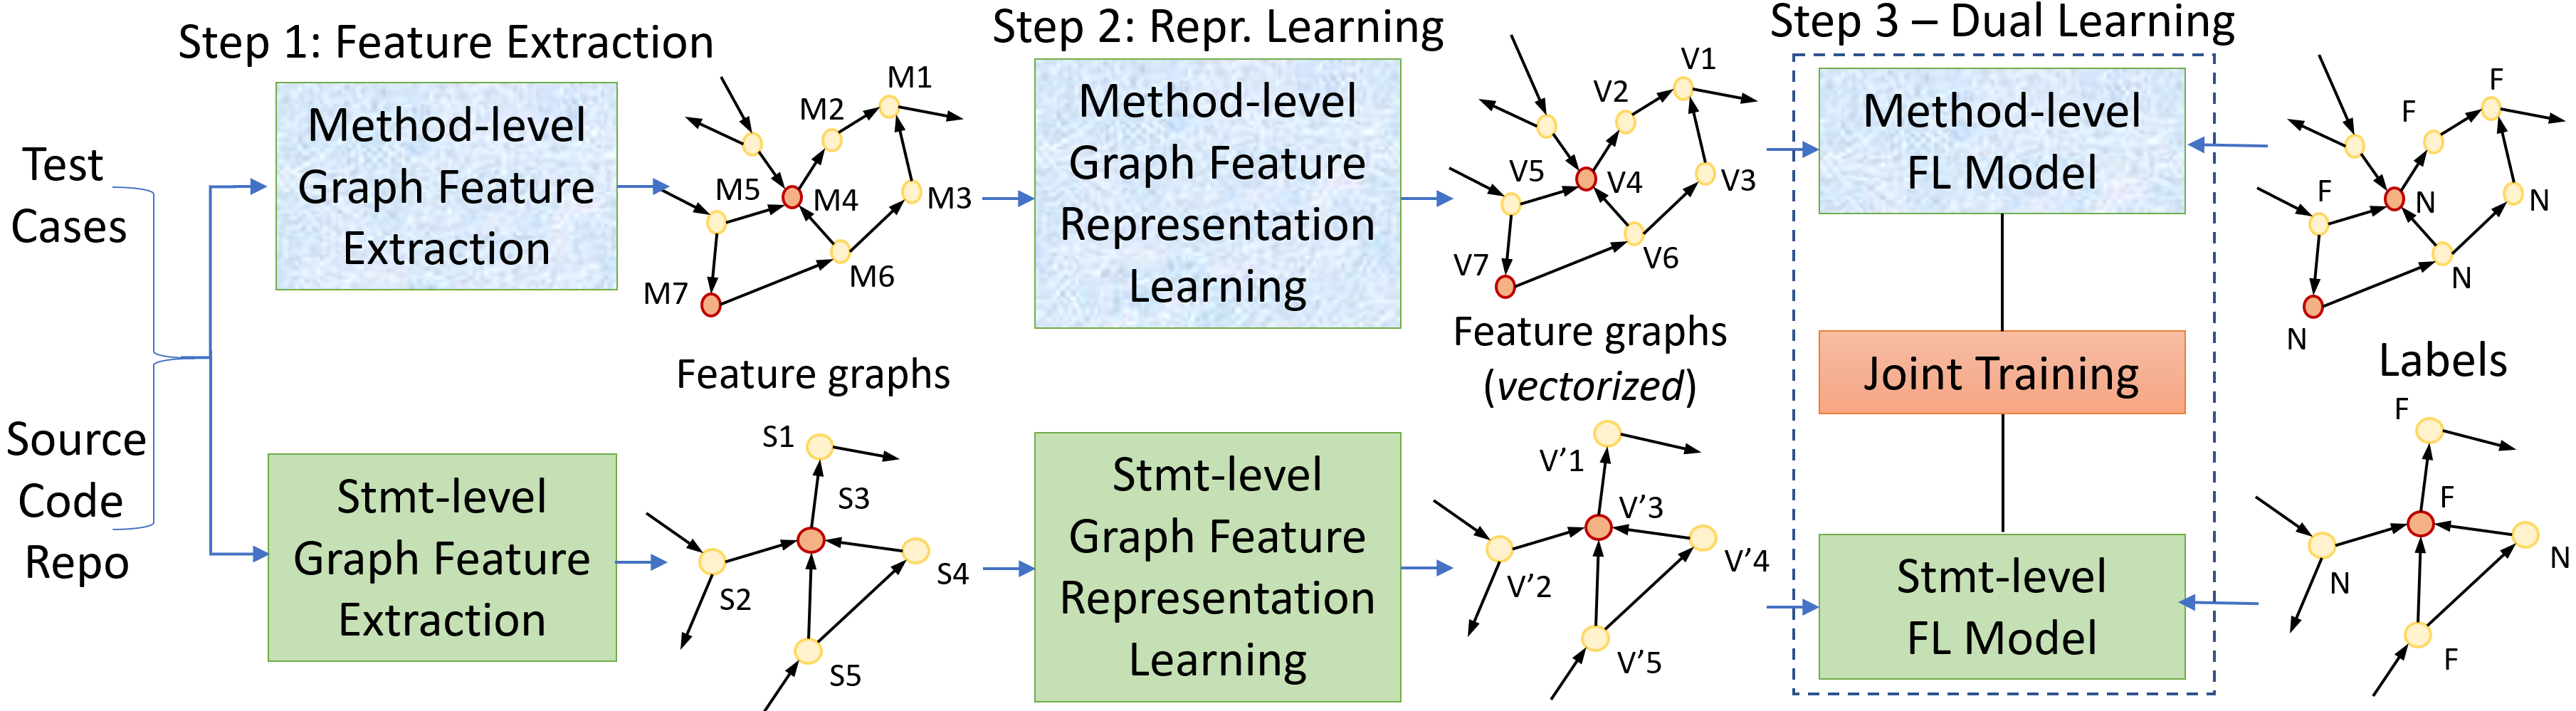
\includegraphics[width=5.45in]{graphs/overview-training.png}
        \vspace{-8pt}
	\caption{{\tool}: Training Process}
        \label{train-overview}
\end{figure*}

\noindent {\bf Observation 1. [Co-Change Fixing Locations]} As seen in
this example, the changes to fix this bug involve multiple faulty
statements that are dependent on one another. Fixing only one of the
faulty statements will not make the program pass the previously
failing test(s). For an APR model to work, an FL tool needs to point
out all of those faulty statements to be changed in the same fix. For
effective manually fixing by developers, an FL tool also needs point
out all faulty statements to be fixed at once. Otherwise, (s)he must
find the missing locations or waste time on incorrect ones.

\noindent {\bf Observation 2. [Multiple Faulty Methods]} As seen, this
bug requires the changes to three different methods at the same time.
It is important for an FL tool to connect and identify these multiple
faulty statements in potentially different methods.

%Traditional FL approaches~\cite{zhang-fse09,ICICA-10} using program
%analysis (PA), e.g., execution flow analysis, could identify all of
%those statements in the same fix due to their caller/callee
%relations.

Traditional FL approaches~\cite{zhang-fse09,ICICA-10} using program
analysis (PA), e.g., execution flow analysis, are restricted to
specific PA techniques, thus, not general to locate all types of CC
fixing locations.
%could identify all of those statements in the same fix due to their
%caller/callee relations.
Spectrum-based~\cite{jones2005empirical,abreu2006evaluation},
mutation-based~\cite{MUSE,papadakis2012using,Metallaxis}),
statistic-based~\cite{liblit-pldi05}, and machine learning (ML)-based
FL approaches~\cite{DeepFL,icse21-fl} could implicitly learn the
program dependencies for FL purpose. However, despite their successes,
the non-PA FL approaches {\em do not support the detection of multiple
  locations that need to be changed in the same fix for a bug, i.e.,
  Co-Change (CC) Fixing Locations}.
%
The spectrum-based and ML-based FL models return a ranked list of
suspicious statements according to the corresponding suspiciousness
scores. In this example, the lines 3, 14, 18, 22, and the other lines
({\em e.g.}, 5, 13, 21 and 25) are executed in the same passing or
failing test cases, thus~assigned with the same scores by
spectrum- and mutation-based FL approaches. A user would not be
informed on what lines need to be fixed together. Those non-PA,
especially ML-based FL approaches, do not have a mechanism to detect CC
fixing locations.

In this work, we aim to advance the level of deep learning (DL)-based
FL approaches to detect CC fixing locations. However, it is not
trivial. A solution of assuming the top-$k$ suspicious statements from
a FL tool as CC fixing locations does not work because even being the
most suspicious, those statements might not need to be changed in the
same fix. In this example, all of the above lines with the same
suspiciousness scores would confuse a fixer.

Moreover, another naive solution would be to use a method-level FL
tool to detect multiple faulty methods first and then use a
statement-level FL tool to detect the statements within each faulty
method. As we will show in our experiment, the inaccuracy of the first
phase of detecting faulty methods will have a confounding effect in
the overall performance in detecting CC fixing statements.



\subsection{Key Ideas}
\label{sec:key-ideas}

To address those challenges, we propose {\tool}, a novel FL approach
to locate all the CC fixing locations (i.e., faulty statements) that
need to be modified in the same fix for a bug. {\tool} has the
following novel key ideas in both new model and features:

{\bf Key Idea 1. [Dual-Task Learning for Fault Localization]} To avoid the
confounding effect in a naive solution of detecting faulty methods
first and then detecting faulty statements in those methods, we design
an approach that treats detecting dependent CC fixing locations as a
{\em dual-task learning} between them. First, the {\em method-level
  FL} model (\code{MethFL}) aims to learn the methods that need
to be modified in the same fix. Second, the {\em statement-level
  FL} model (\code{StmtFL}) aims to learn the co-fixing
statements regardless of whether they are in the same or different
methods.

Intuitively, \code{MethFL} and \code{StmtFL} are related to each
other, in which the results of one model can help the other. We refer
to this relation as {\em duality}, which can provide some useful
constraints for {\tool} to learn dependent CC fixing locations.
%
We conjecture that the joint training of the two models can improve
the performance of both models, when we leverage the constraints of
this duality in term of shared representations. For example, if two
statements in two different methods $m_1$ and $m_2$ were observed to
be changed in the same fix, then it should help the model learn that
$m_1$ and $m_2$ were also changed together to fix the bug.  If two
methods were observed to be fixed together, then some of their
statements were changed in the same fix as well. In our model, we
jointly train \code{MethFL} and \code{StmtFL} with the models'
parameter soft-sharing to exploit their relation. We use a mechanism
called {\em cross-stitch unit}~\cite{misra2016cross} to learn a linear
combination of the input features from two models to {\em enable
  the propagation of the impact of \code{MethFL} on \code{StmtFL} and
  vice~versa}.

%We also add an attention mechanism in the two models to help emphasize
%on the key features.


%Therefore, the third component is the {\em localization model} with
%the main goal of deriving the CC fixing locations. Another task of
%this component is to train the MethFL and StmtFL simultaneously to
%explot the duality. Specifically, we apply a probabilistic correlation
%as a regualization term in the foss function in the join training. We
%also design a novel constraint about the attention mechanism in two
%models.

%two dual regularization terms to constrain the duality of the two
%models, which are enlightened by the probabilistic correlation and the
%symmetry of attention weights between two models.




%{\bf Key Idea 3. [Multi-task Learning Fault Localization]} When doing the fault localization, there are often two levels of fault localization that we can do: the statement-level fault localization and the method-level fault localization. More detailed fault localization can help the developers to find the bugs easier. So for\tool, we regard the statement-level fault localization as our primary goal. However, the method fault localization is still helpful because the method-level fault localization often has higher accuracy and can help reduce the biases. 

%To make the method-level fault localization helpful when doing the statement-level fault localization, in \tool, we build a multi-task learning framework to do the statement-level fault localization. To be more specific, we have two separate models for the two levels of fault localization. The first model is to do the statement-level fault localization as we mentioned in key idea 2. And the second model is to do the method-level fault localization. In this model, we take the method pairs as input and train the model to predict if the method pairs are co-changes or not. During the training process, the parameters between the first and second models are softly shared to build the multi-task learning framework. We will introduce the details in the approach section.

{\bf Key Idea 2. [Co-Change Representation Learning in FL]}~In
detecting CC fixing locations, in addition to a new dual-task learning
model in key idea 1, we use a new feature:
%{\em co-change information}, i.e., the statements/methods that were
%changed together.
{\em co-change information} among statements/methods, which has never
explored in fault localization research.
%
The co-changed statements/methods in the same commit are used to train
the models. We also consider the co-fixed statements/methods in
the same fixes. The rationale for considering general co-changes
is that the co-changed entities in the past might become the ones
that will be fixed together in the future.

%Just as we mentioned in observation 1, co-change is very common when
%we want to fix a bug or do an enhancement on the code. To catch the
%co-change information, we first collect the commits that change the
%source code. And for each commit, we mark the statements that changed
%together as the co-change. By collecting all co-changes from the
%commits in the project, we have a large co-change history
%dataset. Then, to analyze the code relationship, we build a link
%between the statements been changed together. To make the co-change
%information useful, we add these edges into the other graph to do the
%graph modeling. That is our second key idea.

{\bf Key Idea 3. [Graph Modeling for Dependencies among
    Statements/Methods]} The statements/methods that need to be fixed
together are interdependent with several dependencies. Thus, we use
Graph-based Convolution Network (GCN)~\cite{li2019gcn} to model
different types of dependencies among statements/methods,
e.g., data and control dependencies in a program dependence graph
(PDG), execution traces, stack traces, etc.
%For convenience,
We also encode the {\em co-change relations in the same commit or fix}
  among the statements into our graph representations with different
types of edges representing different relations. The GCN model enables
both nodes' and edges' attributes and learns to classify the nodes as
buggy or~not.

%{\bf Key Idea 2. [Multi-edge-types Graph Modeling]}

%As mentioned in observation 2, one bug can be involved in multiple
%methods, and for each method, there can be more than one statement
%related to the bug. To analysis the relationships between the
%statements that in the same method, the graph modeling between the
%source code such as program dependency graph (PDG), execution paths
%(EP), and co-change relationships (CCR) is the way that we thought to
%be suitable. To avoid overlapping, we regard the PDG as the based
%graph, add the EP and CCR edges into the graph, and use the combined
%graph to analyze the relationship.

%However, the different types of edges in one graph cannot be regarded as the same type. To specify the differences among the four different types of edges (PDG contains data dependency and control dependency, two types of edges), we use an advanced GCN \cite{li2019gcn} that takes both node and edge attributes as inputs to learn the node classification. Because it accepts edge attributes, we give the different types of edges with different labels as input to specify their differences.







\section{Approach Overview}
\label{overview:sec}

\begin{figure*}[t]
	\centering
	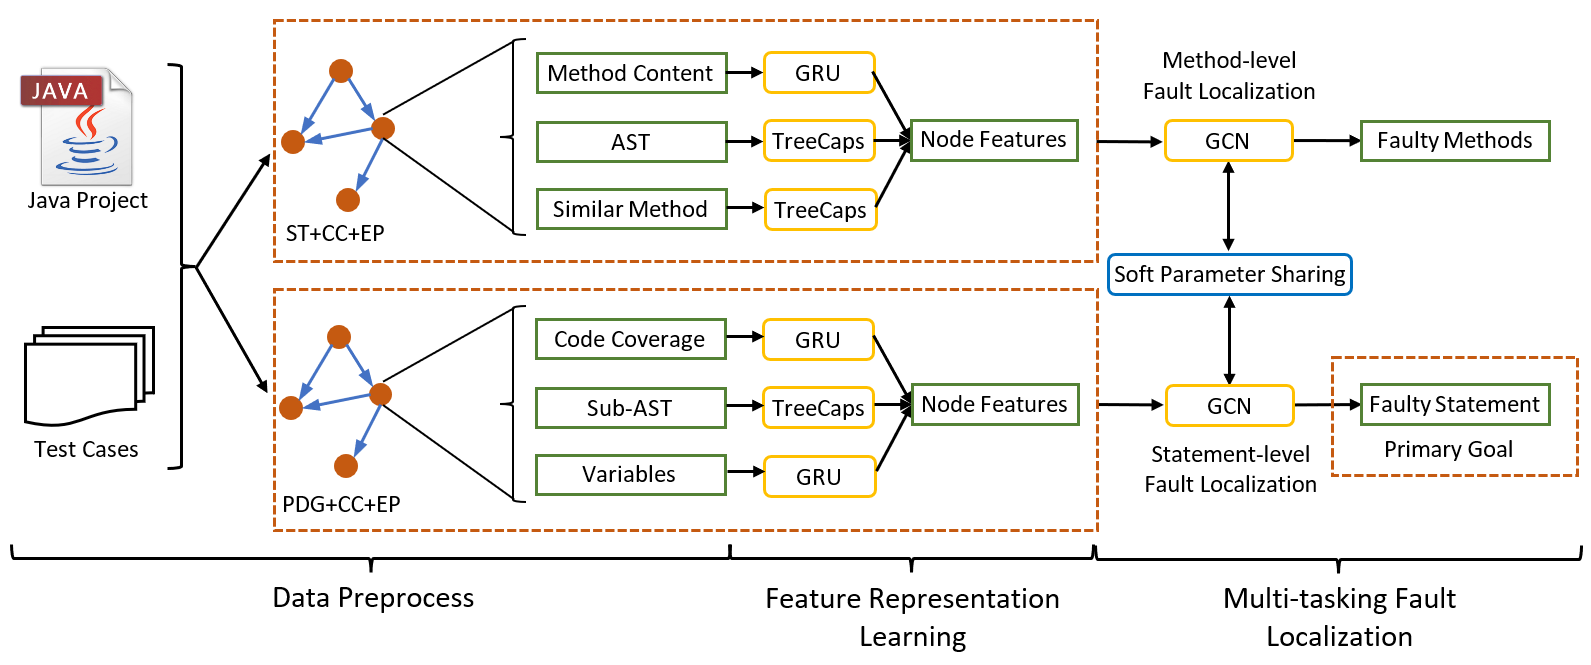
\includegraphics[width=5.4in]{graphs/overview.png}
	\caption{{\tool}: Training Process}
	\label{train-overview}
\end{figure*}

{\tool} has two main processes. Figure~\ref{train-overview} displays the
general architecture of the training process.

\section{Feature Extraction}

The first step of \tool is to preprocess the input data into the suitable format and group them into statement and method two levels. So the input of this step is the \tool input, including the java project that needs to do the fault localization with the commit history and the relevant test cases for the project. And the output of this step is two groups of graphs with node features for statement-level and method-level.

Specifically, \tool extract the features from two levels: the method-level and statement-level feature extraction.

\begin{figure}[t]
	\centering
	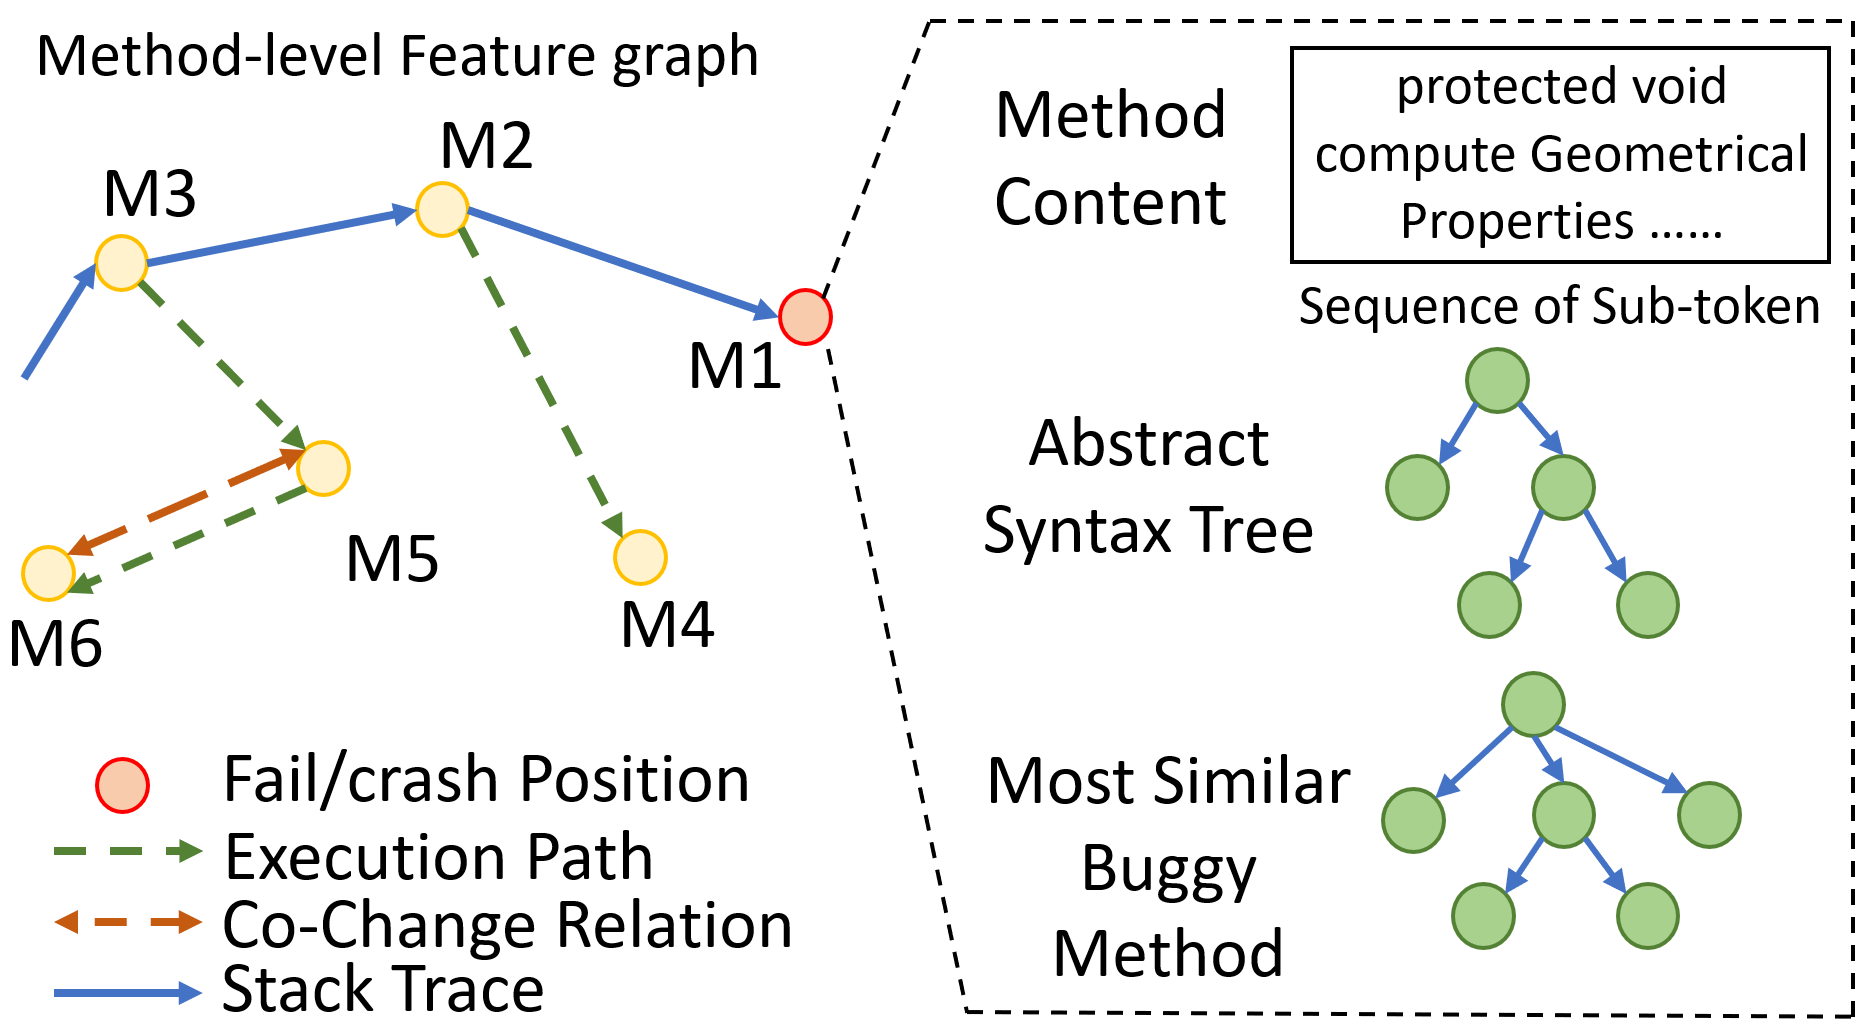
\includegraphics[width=3in]{graphs/step-1-method.png}
	\caption{Method-level Feature Extraction}
	\label{method-level-feature-extraction}
\end{figure}

\subsection{Method-level Feature Extraction}
For the method level, \tool uses the method as the basic unit. And for each method, \tool extracts three key features, including the method content, abstract syntax tree (AST), and the most similar buggy method. 1> For the method content, \tool collect the source code of each method $M$ and link each statement $S_m$ one by one in $M$ as a sequence $Seq_m$ to represent the method content. \tool removes all special characters and uses CamelCase to break down the tokens in the sequence into sub-tokens to reduce the influence of biases. For example, in the Figure \ref{method-level-feature-extraction}, the method content feature in the method $M1$ shows the extracted sequence of sub-tokens $protected void compute ......$. The source code is listed on the input of the Figure \ref{statement-level-feature-extraction}. 2> As for the AST, \tool generates abstract syntax tree $Tree_m$ for each method $M$ by using JDT package \cite{JDT}. The generated AST looks like the example shown on the abstract syntax tree feature in Figure \ref{method-level-feature-extraction}. 3> When extracting the most similar buggy method feature, \tool breaks down the methods into the sequence of sub-tokens just like the method content feature. It then uses GloVe \cite{pennington2014glove} to learn the embedding for each sub-token and replace the sub-tokens with the embedding vectors. After this, \tool calculates the cosine similarity between the current method $m$ and all other buggy methods in the commit history (before the current bug) to find the most similar buggy method $m_b$. For this buggy method, \tool also uses the JDT package to generate the AST for $m_b$. The most similar buggy method feature in Figure \ref{method-level-feature-extraction} shows a possible example for it.

After having these three features for each method, \tool uses three kinds of edges to link them as a graph. First of all, \tool runs test cases for the project. If a test case $t_i$ failed, \tool collect the stack trace for the test case $t_i$. Because the stack trace is sometimes too long, using the crashed position as the root, \tool only picks part of the stack trace $st_i$ with the depth of ten in consideration. It means that on the stack trace $st_i$, there are at most ten methods include $m_1, m_2, ..., m_{10}$ where $m_1$ is the crashed position. For every two method $m_j$ and $m_{j+1}$ among these methods, $m_{j+1}$ calls the $m_j$ in the stack trace. The edge $E_m^s$ direction in it is always from $m_{j+1}$ point to $m_j$. For example, in the Figure \ref{method-level-feature-extraction}, the crashed method is $M1$ and the blue solid edges are the stack trace $st_i$. The figure shows that in the stack trace, $M3$ comes out before $M2$ and $M2$ comes out before $M1$. The second type of edge is the execution path. By using each method $m_j$ in the stack trace $st_i$ as the root method, \tool expands the stack trace $st_i$ by adding the executed methods into the graph. The direction of the execution edges $E_m^e$ is also the same as the call direction. Also, because sometimes the execution path may be very long for a method, we only keep the methods $m_k$ within ten steps from the crashed position $m_1$ that means in the graph, from node $m_k$ to $m_1$, the steps are no more than ten (when counting the steps, \tool ignore the edge direction). The green dotted line in Figure \ref{method-level-feature-extraction} shows an example for this type of edge. With the Figure \ref{method-level-feature-extraction}, the green dotted line reflects the relationship that when running the test case $t_i$ on $M2$, it also executes the method $M4$ based on the method call. And then, it executing the $M3$, it executes the method $M5$, and within $M5$, it also executes method $M6$ based on the method calls inside the methods. The third type of edge is the co-change relation. For this,  \tool collects all commit history from the input java project. If more than one method has changed in one commit, we mark it as a co-change. The co-change contains all the methods that changed together in this commit. To add the co-change relation as one type of edge, \tool makes the co-change relation become a two-directional edge $E_m^c$ (e.g. The orange edge between $M5->M6$ and $M6->M5$ in the Figure \ref{method-level-feature-extraction}).
%
%\begin{itemize}%
%	\item Graph: 
%	\begin{itemize}
%		\item Stack Trace: \tool runs test cases for the project. If a test case $t_i$ failed, \tool collect the stack trace for the test case $t_i$. Because the stack trace may be very bug, by using the crashed position as the root, \tool pick part of the stack trace $st_i$ with the depth of ten. It means that on the stack trace $st_i$, there are ten methods include $m_1, m_2, ..., m_{10}$ where $m_1$ is the crashed position and for every two method $m_j$ and $m_{j+1}$ among them, $m_{j+1}$ calls the $m_j$ in the stack trace. The edge $E_m^s$ direction in it is always from $m_{j+1}$ point to $m_j$ \tool uses $st_i$ as the base graph and the relationship information in $st_i$ is the dynamic information. 
%		\item Execution Path: As for the failed test case $t_i$, \tool also analyzes the execution path. By using each method $m_j$ in the stack trace $st_i$ as the root method, \tool expands the stack trace $st_i$ by adding the executed methods into the graph. The direction of the execution edges $E_m^e$ is also the same as the call direction. Also, because sometimes the execution path may be very long for a method, we only keep the methods $m_k$ within ten steps from the crashed position $m_1$ that means in the graph, from node $m_k$ to $m_1$, the steps are no more than ten (when counting the steps, \tool ignore the edge direction). The added execution information here is the dynamic edge.
%		\item Co-change Information: \tool collects all commit history of the input java project. If more than one java method has changed in one commit, we mark it as a co-change. The co-change contains all the methods that changed together in this commit. Because the co-change does not have the direction, there is one non-directional edge $E^c$ between every two methods in this co-change to represent the co-change relationship. In order to add the co-change relationship into the stack trace, \tool makes the non-directional edge $E^c$ become a two-directional edge $E_m^c$ (e.g.$method_A -> method_B$ and $method_B -> method_A$). This type of edge is the static edge.
%	\end{itemize}
%	\item Node Features: 
%	\begin{itemize}
%		\item Method Content: \tool collect the source code of each method $M$ and link each statement $S_m$ one by one in $M$ as a sequence $Seq_m$ to represent the method content. \tool removes all special characters and uses CamelCase to break down the tokens in the sequence into sub-tokens to reduce the influence of biases. For example, the $setTagAsStrict$ can be break down into $set, Tag, As,$ and $Strict$. The processed sequence of sub-tokens $Seq^p_m$ is used to represent the method content in \tool. This feature is one of the static features that \tool collects from the source code to represent the method.
%		\item Method Structure: \tool generates abstract syntax tree $Tree_m$ for each method $M$ by using JDT package \cite{JDT}. Each tree $Tree_m$ represent the structure of the relevant method $m$. This is one of the static feature that \tool collect from the source code to represent the method.
		%\item Similar Buggy Method: \tool breaks down the methods into the sequence of sub-tokens just like method content feature and then uses GloVe \cite{pennington2014glove} to learn the embedding for each sub-token and replace the sub-tokens with the embedding vectors. After this, \tool calculate the cosine similarity between the current method $m$ and all other buggy methods in the commit history (before current bug) to find the most similar buggy method $m_b$. This is one of the static feature that \tool collect from the source code to represent the method.
%	\end{itemize}	
%\end{itemize} 


\begin{figure}[t]
	\centering
	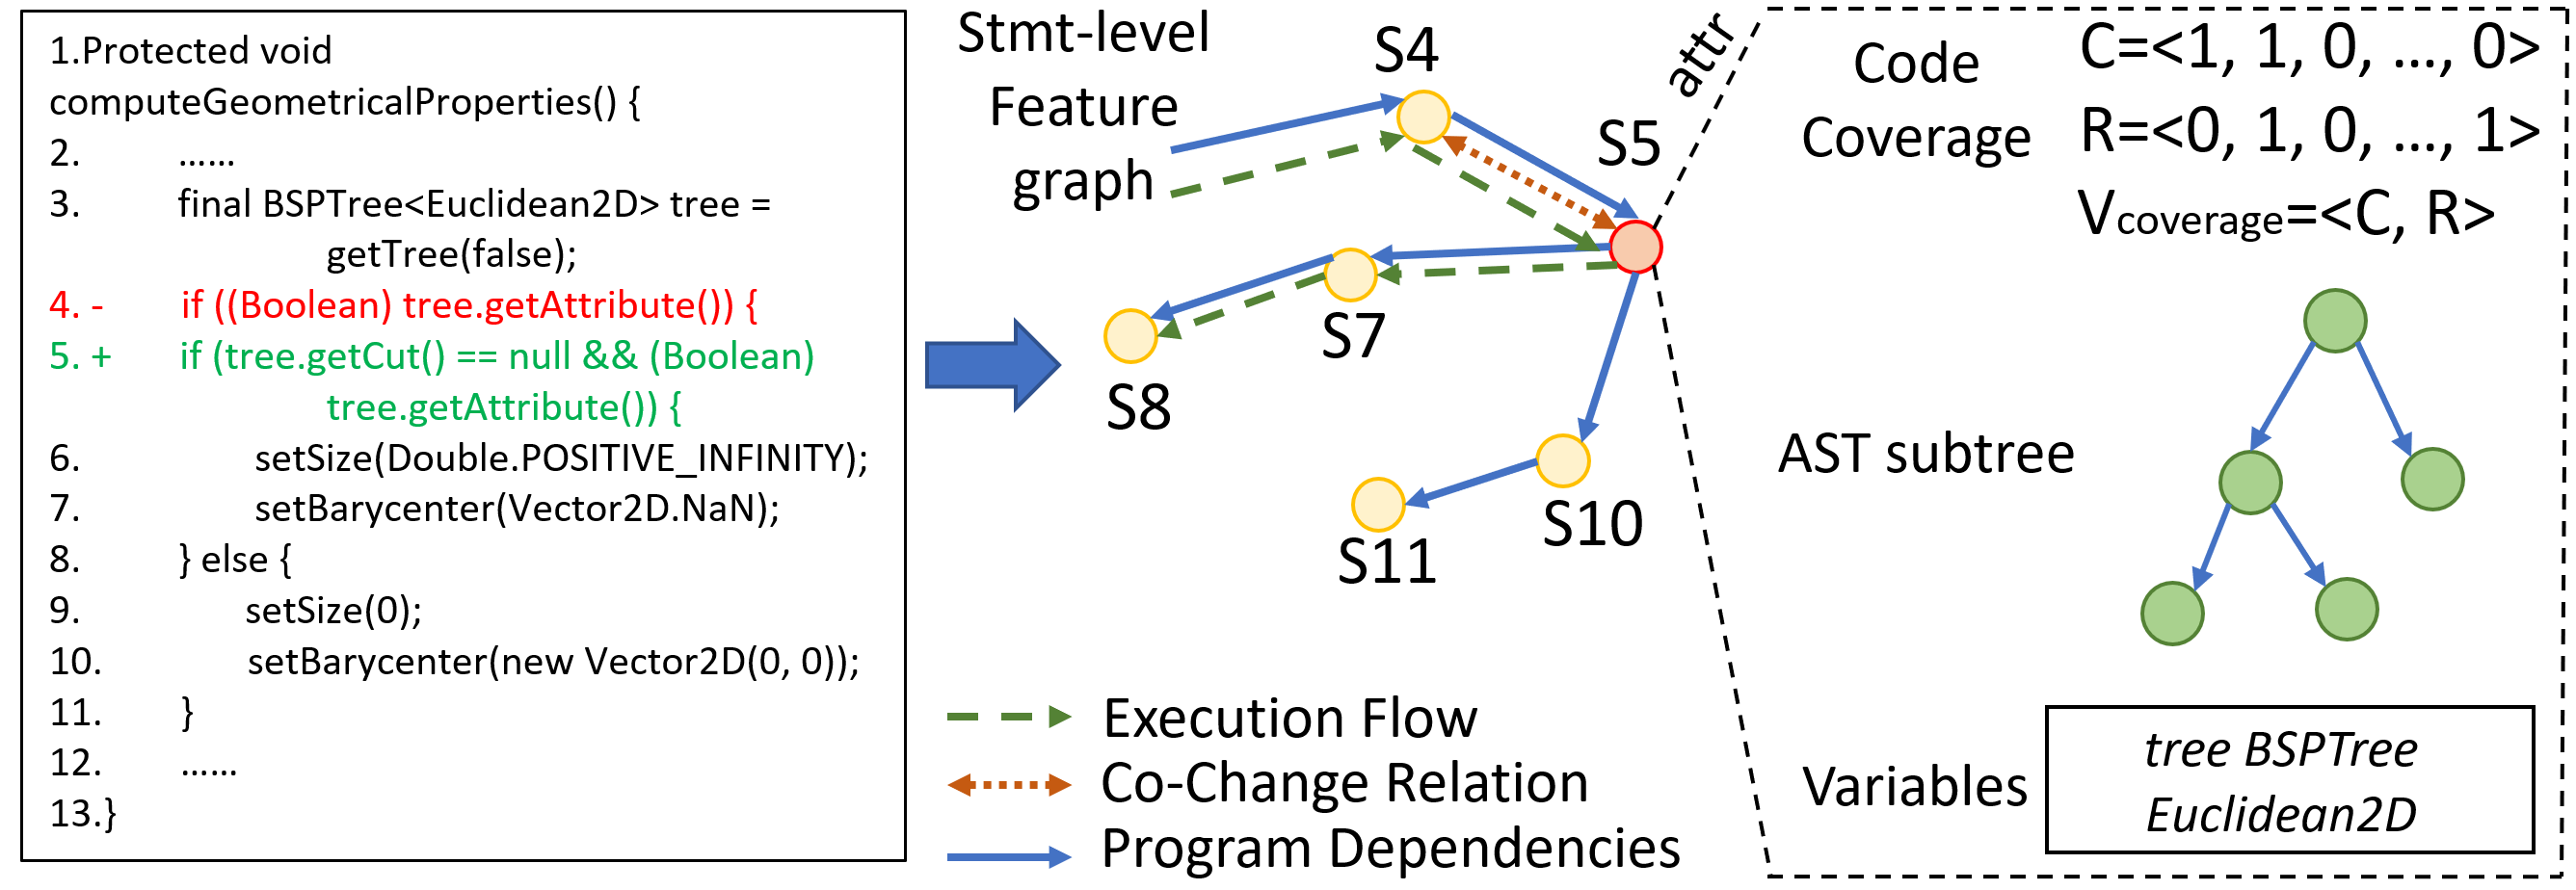
\includegraphics[width=3.4in]{graphs/step-1-statement.png}
	\caption{Statement-level Feature Extraction}
	\label{statement-level-feature-extraction}
\end{figure}

\subsection{Statement-level Feature Extraction}

For the statement level,  \tool uses the statement as the basic unit. And for each statement, \tool extracts three key features, including the code coverage information, sub-AST, and variables to represent the statement. 1> As for the code coverage information, \tool runs the relevant test cases for the input project. For the test case $t_i$, if it passes the statement $s_i$, \tool uses $c_i = 1$ to represent it while if it does not pass the statement $s_i$, \tool uses $c_i = 0$ to represent it. By linking all $c_i$ together, \tool can get $C = <c_1, c_2, ..., c_i>$. Also, \tool uses $r_i = 1$ to represent the the condition $passed$ and uses $r_i = 0$ to represent the condition $failed$ for the test case $t_i$ . By linking all $r_i$ together, \tool can get $R = <r_1, r_2, ..., r_i>$. By concatenate $C$ and $R$, \tool extract the code coverage information feature by $V_{coverage} = <c_1, c_2, ..., c_i, r_1, r_2, ..., r_i>$. The code coverage information feature in Figure \ref{statement-level-feature-extraction} shows an example of it. 2> For the sub-AST, it is very similar to the method level. By using JDT package, \tool can extract the AST for the whole method. And then, \tool searches for the nodes that appears in the statement. By collecting all these nodes and the edges between then, \tool can extract the sub-AST for the statement. 3> For the variables feature, for each statement, \tool collects all the variables $V$ that appeared in it and for each variable $v$ in $V$, \tool uses the $(variable_name variable_type)$ to represent it. Then \tool links all variables $V$ together with $,$ as a sequence $Seq_s$ as one of the static feature that \tool collect from the source code to represent the statement. For example, in Figure \ref{statement-level-feature-extraction}, \tool goes through the statement at $line 5$ in the input method and finds that only one variable $tree$ appears in the statement at $line 5$. So the variable feature here should be like $variable_name variable_type$ where $variable_name$ is $tree$ and $variable_type$ is $BSPTree Euclidean2D$.

With these three features, similar to the method-level, \tool builds three types of edges to link the statements together as a graph. The first type of edge is the program dependency edge (PD). \tool builds the PD by using the tool soot \cite{soot} for the method $m$. For example, in Figure \ref{statement-level-feature-extraction}, the blue edges are the PD edges and they show that in method $m$, statement at $line 4$ controls the statement at $line 5$. And statement at $line 5$ can control the statements at $line 7-8$ and the statements at $line 10-11$. The second type of edge that \tool extracts is the execution flow $E_s^e$. The execution flow is the order that the failed test case $t_i$ went through in the method $m$. For example, the green dotted edges are the execution flow. Within it, we can see that the test case executes $S7-S8$ but did not go through $S10-S11$. Even though in the PD, $S5$ is linked by $S10-S11$. It means that when running the test case $t_i$, it will not pass the $S10$ and $S11$ because of the if checking in $S5$. The last type of edge $E_s^c$ is the co-change relation in the statement level. \tool collects the co-change information for the commit about the statements that changed together before in the current method $m$ and one commit. In Figure \ref{statement-level-feature-extraction}, the commit history shows that $S4$ and $S5$ used to be changed together before. Hence, there is an orange edge that represents the co-change relation between $S4$ and $S5$.


%\begin{itemize}
%	\item Graph: 
%	\begin{itemize}
	%	\item Program Dependency Graph (PDG): \tool builds the PDG by using the tool soot \cite{soot} for the method $m$ that contains the statements that \tool want to analyze. \tool uses the generated PDG as the base graph. Within this graph, there are two types of edges including data dependency and control dependency. Both of these two types of edges are the static edges.
	%	\item Execution Path: \tool collects the execution path of the failed test case $t_i$ within the method $m$ and adds them into the PDG by adding a new type of edge $E_s^e$. The new edge direction is the same as the execution order. This type of edge is the dynamic edge.
%		\item Co-change Information: Similar to the method-level, \tool collects the co-change information for the commit about the statements that changed together before in one commit and the current method $m$. As for adding the co-change information into the PDG, \tool also creates the two-directional edge $E_s^c$ similar to the method level. This type of edge is the static edge.
%	\end{itemize}
%	\item Node Features: 
%	\begin{itemize}
	%	\item Code Coverage Information: \tool runs the relevant test cases for the input java project. For the test case $t_i$, if it passes the statement $s_i$, \tool uses $c_i = 1$ to represent it while if it does not pass the statement $s_i$, \tool uses $c_i = 0$ to represent it. By linking all $c_i$ together as $C = <c_1, c_2, ..., c_i>$, $C$ is considered by \tool as one of the dynamic feature.
	%	\item Statement Structure: Similar to the method-level, \tool generates a sub abstract syntax tree $Tree_s$ for each statement $S$ by using JDT \cite{} package. Each tree $Tree_s$ represent the structure of the relevant statement $s$. This feature is one of the static features that \tool collects from the source code to represent the statement.
	%	\item Variables: For each statement, \tool collects all the variables $V$ that appeared in it and for each variable $v$ in $V$, \tool uses the $(variable_name variable_type)$ to represent it. Then \tool links all variables $V$ together with $,$ as a sequence $Seq_s$ as one of the static feature that \tool collect from the source code to represent the statement. For example, the variables in the statement in line 3 in Figure \ref{fig:motiv} include $root$ and $sourceMap$. \tool generates the feature for them as $root Node, sourceMap SourceMap$ where $root$ and $sourceMap$ are the names and $Node$ and $SourceMap$ are the types.
%	\end{itemize}	
%\end{itemize} 

\section{Feature Representation Learning}
\label{feature-learning:sec}

The goal of this step is to learn to build the vector representations
for the nodes in the feature graph at the method and statement levels.
At each level, the input is the attributes of either a method or a
statement as in Figures~\ref{method-level-feature-extraction} and
~\ref{statement-level-feature-extraction}. The output is each feature
graph in which the nodes are replaced by their embeddings.

%In this step, \tool aims to learn the node feature embeddings based on the node features generated from step 1. So the input of this step is the method-level and statement-level graphs, and the expected output is the node embedding vectors for each node in each graph.

%To be more detailed, we also introduce the node feature representation learning from both method-level and statement-level.

\subsection{Method-level Representation Learning}

\begin{figure}[t]
	\centering
	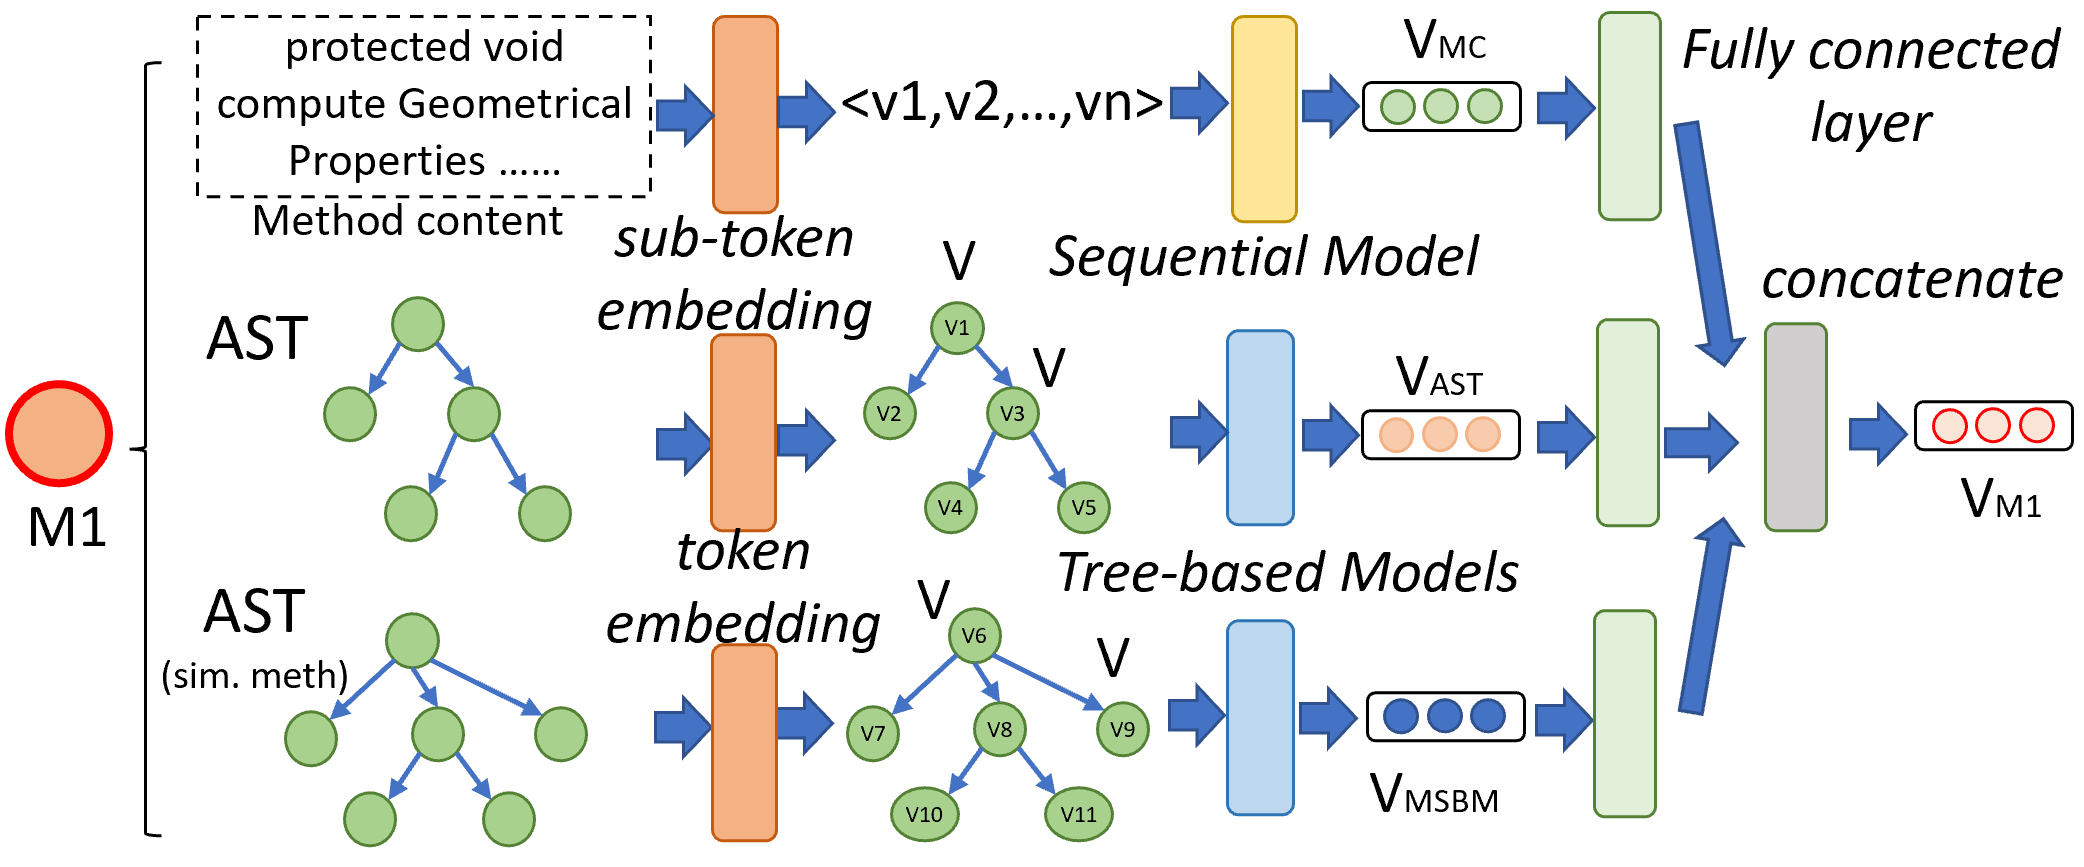
\includegraphics[width=3.4in]{graphs/step-2-method-new.png}
	\caption{Method-level Feature Representation Learning}
	\label{method-level-feature-learning}
\end{figure}

%From step 1, for each node representing a method $M$, there are extracted sequences of sub-tokens $Seq^p_m$ as the method content, generated AST $Tree_m$, and the generated AST for the most similar buggy method $M_b$ as the node features. Thus, to learn the feature representation, we follow these steps.

1) {\em \underline{The method's content}}: the method's content is
represented by the sequence $Seq_c$ of the sub-tokens of the program
elements found in the method's interface and body. To capture the
meaning of each sub-token in $Seq_c$, we use a word embedding model,
called GloVe~\cite{glove2014} to run on $Seq_c$. After this
vectorization, from the sequence $<v_1,v_2, ..., v_n>$ of the vectors
for all the sub-tokens in $Seq_c$, we use a sequential model to learn
the ``summarized'' vector $V_{MC}$ that represents the method's
content. Specifically, we use Gated Recurrent Unit
(GRU)~\cite{cho2014learning}, a type of the RNN layer that is efficient in
learning and capturing the information in the sequence.

%1) {\em \underline{The method's content}}: \tool uses the token embedding techniques to learn the representation vector for each token in the sequence and then replace each sub-token with the embedding vector generated from the techniques. The GloVe \cite{pennington2014glove} is a good word embedding technique that can catch the meaning of the sub-token well, so \tool uses GloVe as the token embedding technique. After the vectorization, \tool has a sequence of vector $Seq^{pe}_m$ and then uses a sequential model to learn the summarized vector that can represent the method's content.  GRU layer \cite{cho2014learning} is a type of RNN layer that is efficient in learning and summarizing the information in the sequences. \tool uses the GRU layer here to learn the embedding vector $V_{mc}$ for the method content. For example, as you can see in Figure \ref{method-level-feature-learning}, the method content first goes through the sub-token embedding bar and become a sequence of vectors. Each vector inside represents a sub-token. Such as $V_{geometrical}$ represent the sub-token $geometrical$. And then, this sequence is feed into the sequential model and gets the $V_{mc}$ as a summary to represent the method content.

2) {\em \underline{The method's structure}}: we first treat the
method as the sequence of tokens and use GloVe to build
the embeddings for all the tokens as in 1). We then replace every node
in the AST of the method with the GloVe's vector of the corresponding
token of the node (Figure~\ref{method-level-feature-learning}).  From
the tree of vectors, we use a tree-based model, called
TreeCaps~\cite{bui2021treecaps}, to capture its structure to
produce the ``summarized'' vector $V_{AST}$ representing the entire
method's~structure.

%Similarly, \tool firstly uses the GloVe to vectorize the AST just as in 1) and then uses a tree-based model to learn the method's structure. One of the most recent studies, TreeCaps \cite{bui2021treecaps} proves that it is good at learning the tree structure information. So \tool uses TreeCaps as the tree-based model to learn the embedding vector $V_{AST}$ to catch the tree structure information. As shown in Figure \ref{method-level-feature-learning}, the generated AST firstly has been vectorized with GloVe and then use the tree-based model to get the representation vector $V_{AST}$

3) {\em \underline{Most similar buggy method}}: for each method, we
keep the most similar buggy one $M_b$. We process $M_b$ in the same
way as the method's structure via GloVe and TreeCaps to learn the
embedding vector $V_{MSBM}$ to represent $M_b$.

%As for the similar buggy method, \tool doing the same process as the method structure feature by using the GloVe and TreeCaps to learn the embedding vector $V_{MSBM}$. Similar as feature 2), in figure \ref{method-level-feature-learning}, the bottom line shows how the vector $V_{MSBM}$ generated for method $M1$

\subsection{Statement-level Representation Learning}

\begin{figure}[t]
	\centering
	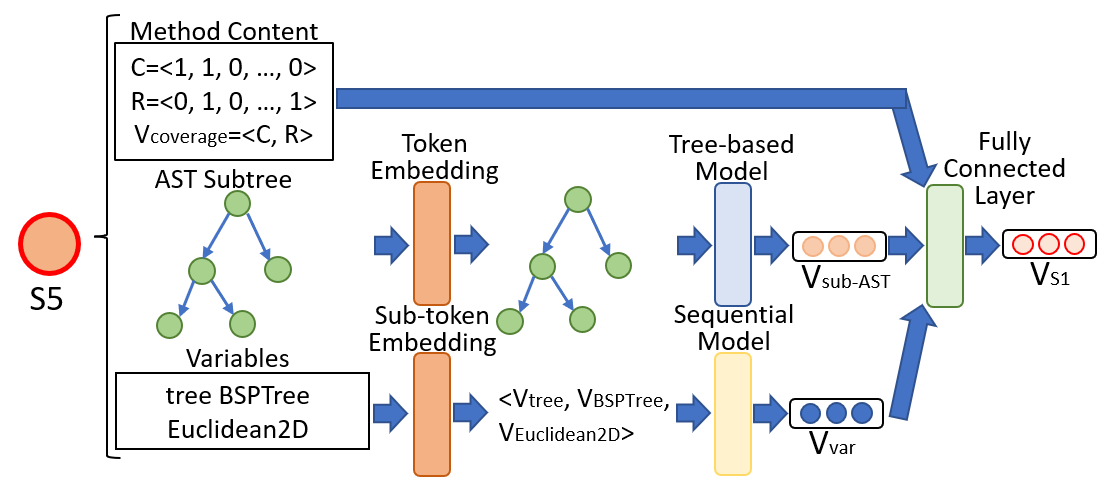
\includegraphics[width=3.4in]{graphs/step-2-statement-new.png}
	\caption{Statement-level Feature Representation Learning}
	\label{statement-level-feature-learning}
\end{figure}

From step 1, for each node representing a statement $S$, there are extracted code coverage information vector, generated AST subtree $Tree_s$, and the generated variable sequence as the node features. Thus, to learn the feature representation, we follow these steps.

1) {\em \underline{Code Coverage}}: \tool does not make any changes and directly regard $V_{Cov} = <c_1, c_2, ...,
c_K, r_1, r_2, ..., r_K>$ that is extracted from step 1 as the embedding vector $V_{cc}$ for the code coverage. 

2) {\em \underline{The statement's structure}}: \tool does the same process as the method's structure feature. \tool firstly using the GloVe to vectorize the AST and then using tree-based model TreeCaps to learn the embedding vector $V^{subtree}$. Just like the process steps for the AST subtree feature in Figure \ref{statement-level-feature-learning}.

3) {\em \underline{List of variables}}: As for the similar buggy method, \tool doing the same process as the method structure feature by using the GloVe and TreeCaps to learn the embedding vector $V^{var}$. For example, in Figure \ref{statement-level-feature-learning}, the variable sequence $tree BSPTree Euclidean2D$ in $S5$ has been embedded through the sub-token embedding technique into $<V_{tree}, V_{BSPTree}, V_{Euclidean2D}>$ and then the sequential model learns the representation vector $V_{var}$ for the variable sequence. 

After having the six embedding vectors mentioned above, \tool uses six fully connected layers to standardize each embedding vector's length to $l/3$ (Here l/3 is an integer). And then, for both method-level and statement-level, \tool concatenate three feature embedding vector into one vector $V_{M}$ or $V_{S}$ for the method-level or statement-level with the length of $l$. In this case, for both method-level and statement-level, \tool all has the graph $G_m$ or $G_s$ with the node embedding vector $V_{m}$ or $V_{s}$. It is the input for the next step.


\section{Dual-Learning Fault Localization}

\begin{figure}[t]
	\centering
	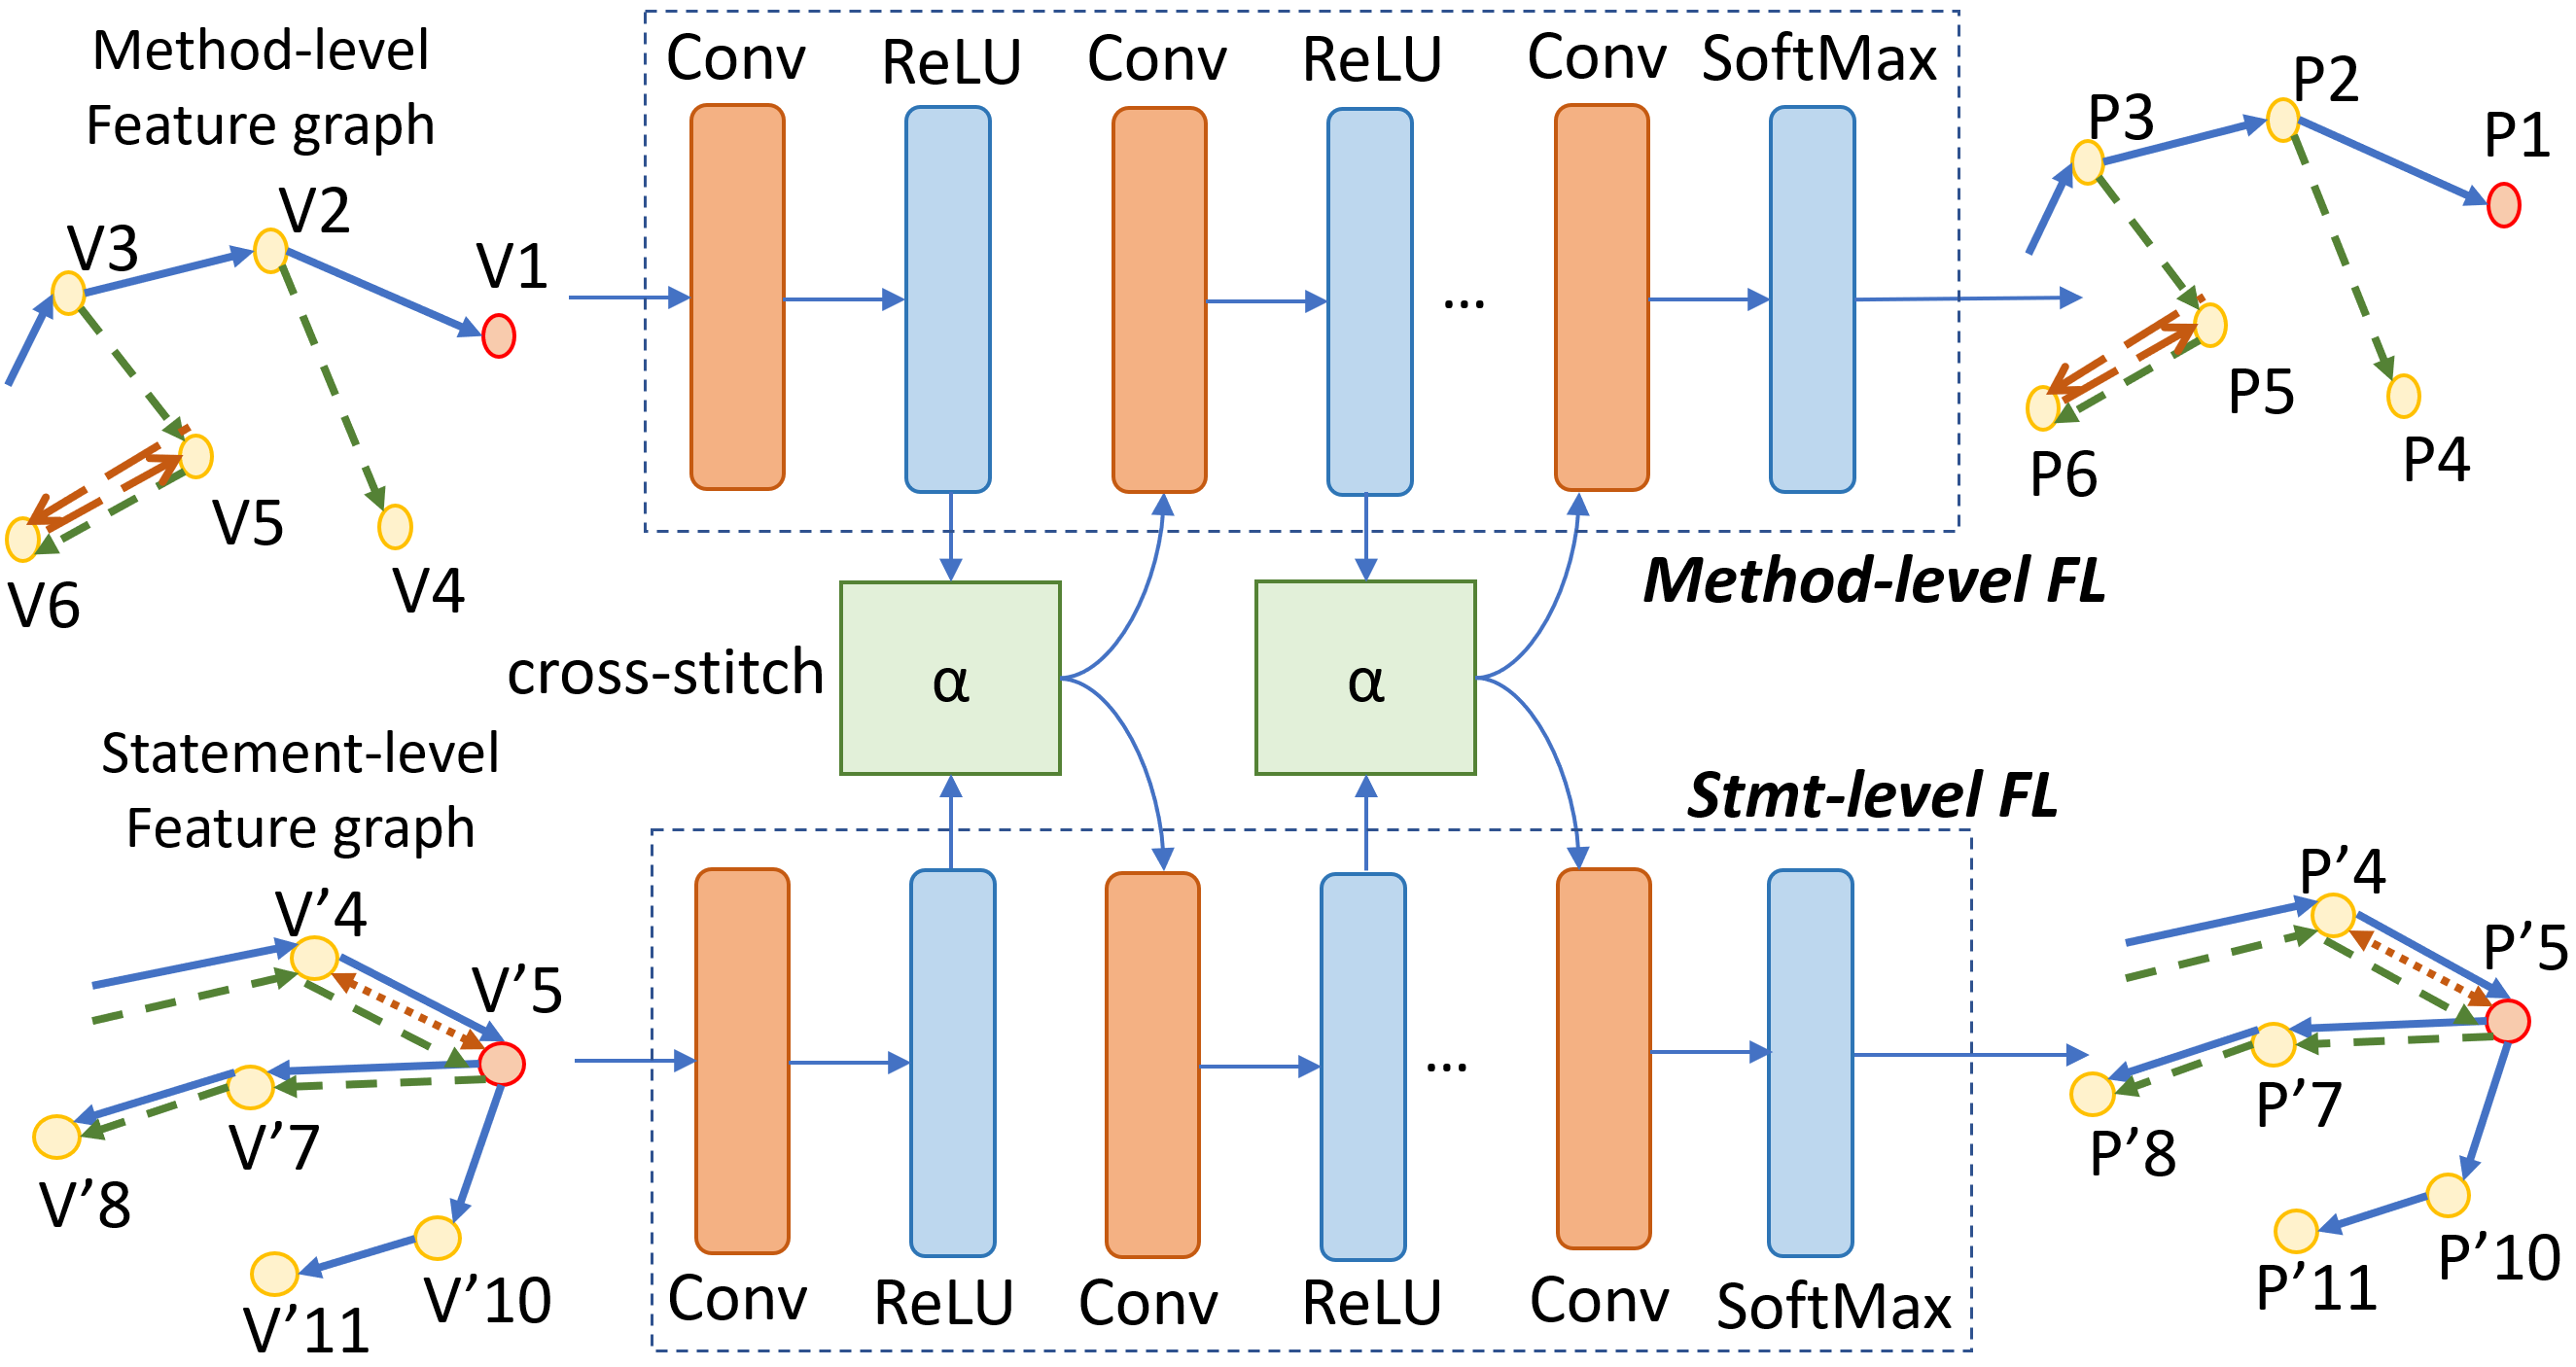
\includegraphics[width=3.4in]{graphs/dual-learning.png}
	\caption{Dual-Learning Fault Localization}
	\label{dual-learning}
\end{figure}

\begin{figure}[t]
	\centering
	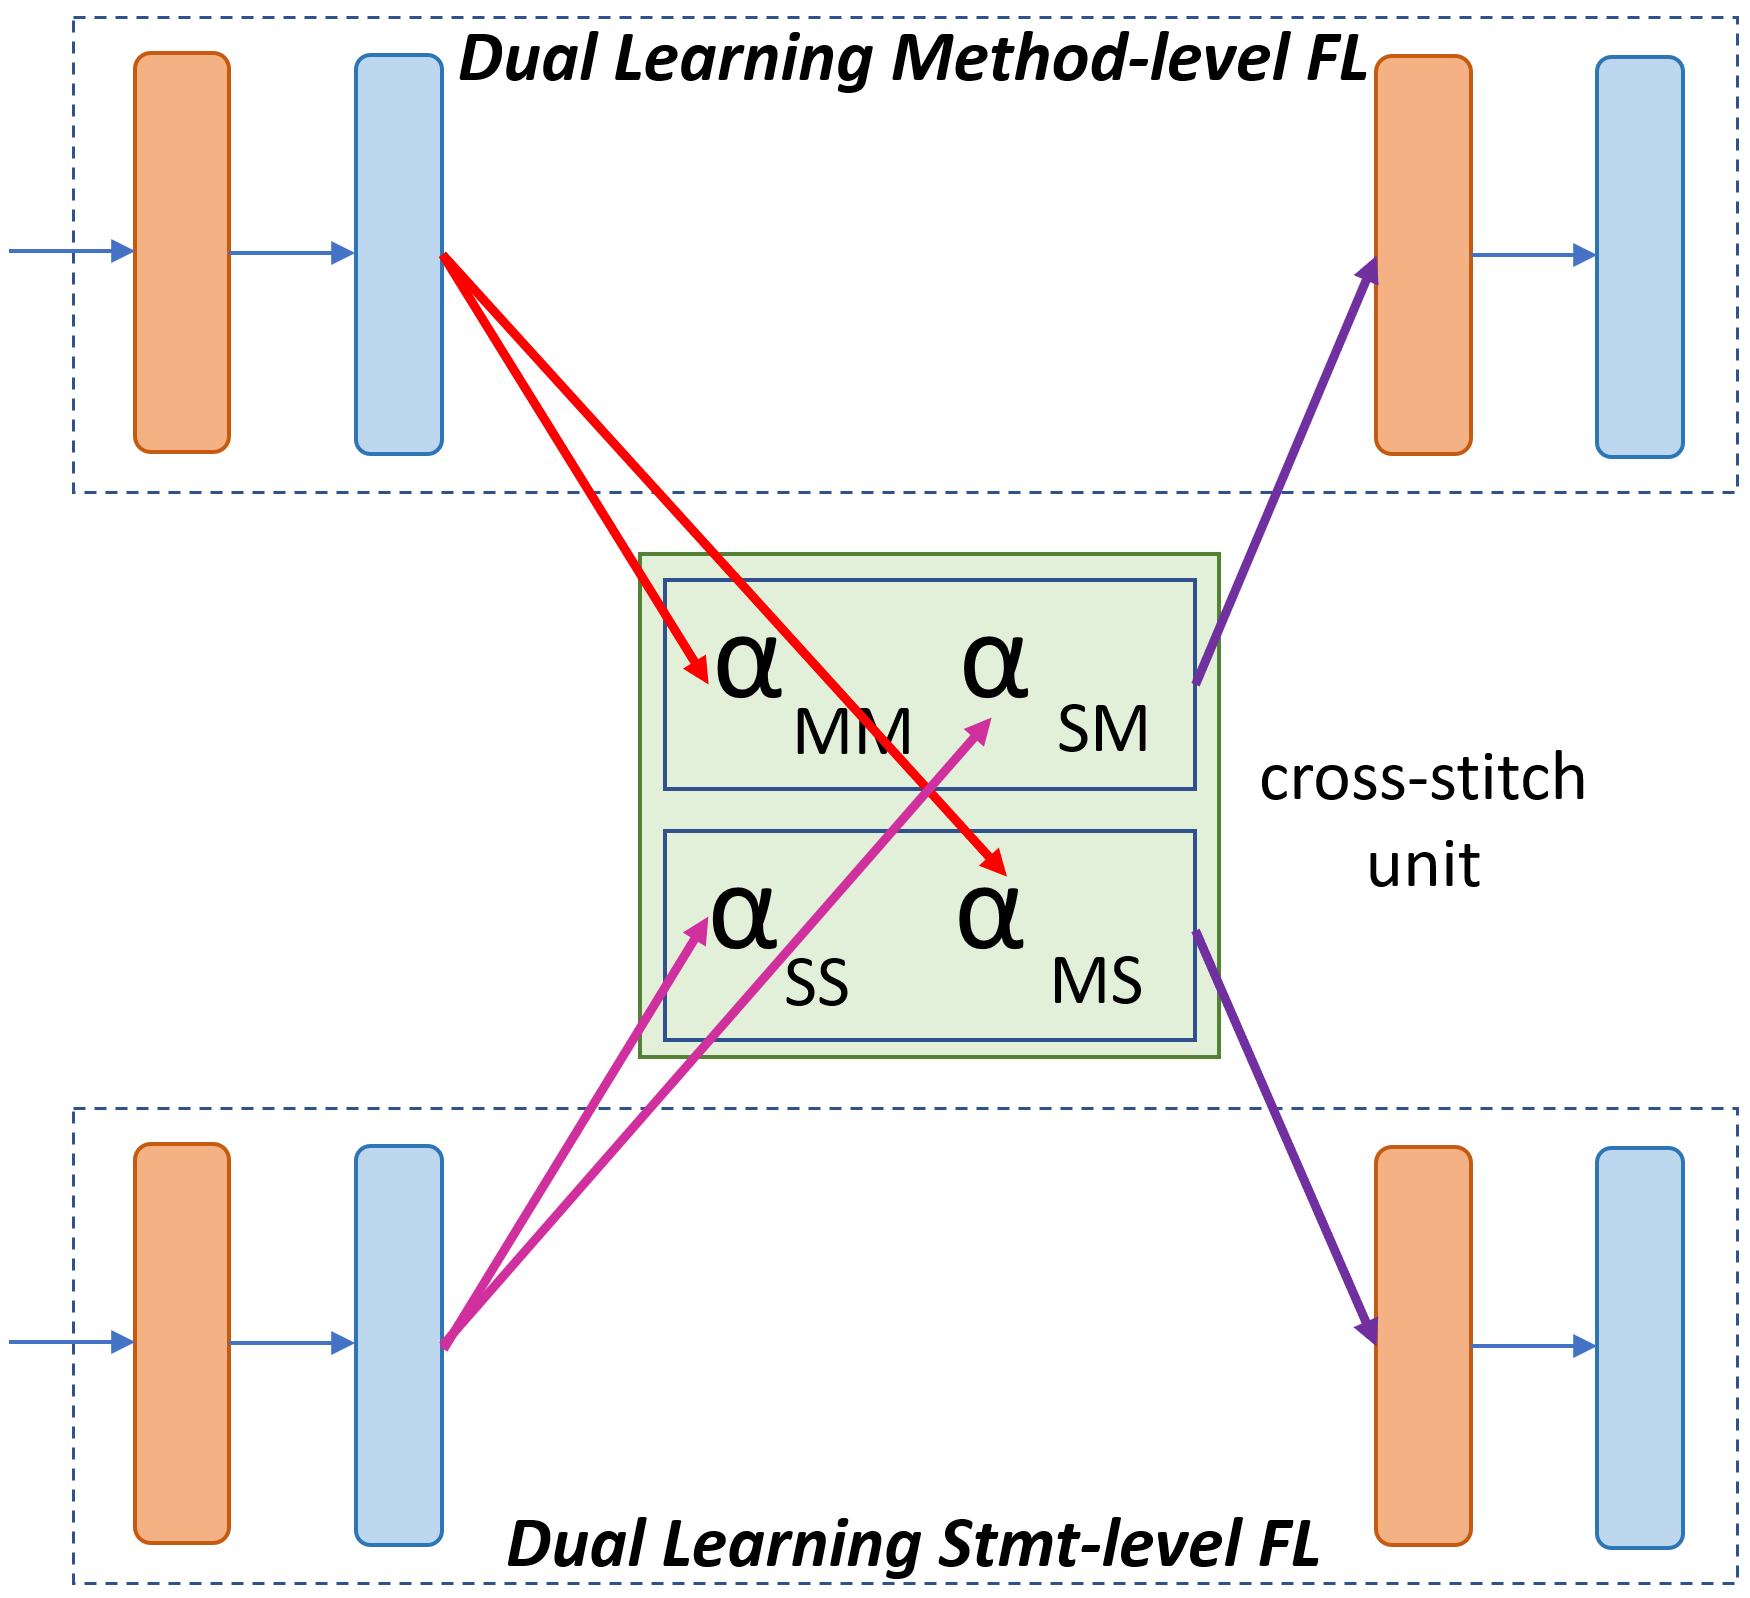
\includegraphics[width=2in]{graphs/cross-stitch.png}
	\caption{Dual Learning via Cross-stitch Unit}
	\label{cross-stitch}
\end{figure}

This section explains our dual learning scheme in step 3 (illustrated
in Figures~\ref{dual-learning} and~\ref{cross-stitch}). The input of
this step includes two feature graphs $G_M$ and $G_S$ for the method
and statement levels. Each node in each feature graph is a vector
computed for a method or a statement (explained in
Section~\ref{feature-learning:sec}). The output is the output graphs
for methods and statements. For the training process, each node in an
output graph has a buggy or non-buggy label.  For the prediction, each
node in an output graph will be predicted as buggy or non-buggy.

%After having the vectorized graph $G_m$ and $G_s$ for both the method-level and the statement-level features,

%in this step, \tool applies a dual learning fault localization model to extract the fault locations. So there are two main tasks in this step, including the method-level fault localization and the statement-level fault localization. So the input for this step is the two graphs $G_m$ and $G_s$, and the expected output is the prediction label for each node in these two graphs from these two tasks.

%Tien
\noindent {\bf Graph Convolution Network (GCN) for FL.} First, {\tool}
has two GCN models~\cite{kipf2016semi}, each for FL at the method and
statement levels. Each GCN model has $n-1$ pairs of a graph
convolution layer (\code{Conv}) and a rectified linear unit
(\code{ReLU}). They are aimed to consume and learn the characteristic
features in the input feature graph. The last pair of each GCN model
is a pair of a graph convolution layer (\code{Conv}) and a softmax
layer (\code{SoftMax}). The \code{SoftMax} layer plays the role of the
classifier on whether a node corresponding to a method or a statement
is labeled as buggy or non-buggy.

\noindent {\bf Dual Learning with Cross-stitch Unit.} In a regular GCN
model, those above pairs of \code{Conv} and \code{ReLU} are connected
to one another. However, to achieve dual learning between method-level
and state\-ment-level FL (\code{methFL} and \code{stmtFL}), we apply a
cross-stitch technique~\cite{misra2016cross} to connect the two GCN
models. The sharing of representations between \code{methFL} and
\code{stmtFL} is modeled by learning a linear combination of the input
features in both feature graphs. At each of the \code{ReLU} layer of
each GCN model (Figure~\ref{cross-stitch}), we aim to learn such a
linear combination of the output from the graph convolution layer
(\code{Conv}) of \code{methFL} and \code{stmtFL} models.

The top sub-network in Figure~\ref{dual-learning} gets direct
supervision from \code{methFL} and indirect supervision (through
cross-stitch units) from \code{stmtFL}~\cite{misra2016cross}.
Cross-stitch units help regularize both tasks \code{methFL} and
\code{stmtFL} by learning and enforcing shared representations by
combining feature maps~\cite{misra2016cross}.


%Tien
%The α values of a cross-stitch unit model linear combinations of
%feature maps. Their initialization in the range [0, 1] is important
%for stable learning, as it ensures that values in the output
%activation map (after cross-stitch unit) are of the same order of
%magnitude as the input values before linear combination.
%-----

\noindent {\bf Formulation.} Let us explain the mathematic foundation
of this scheme. For each pair of the GCN model, the outputs of the
\code{ReLU} layer, called the hidden states, are computed as follows:
\begin{equation}\label{eq:1}
	\hat{A} = D'^{-\frac{1}{2}}A'D'{-\frac{1}{2}}
\end{equation}

\begin{equation}\label{eq:2}
	H_i = \Delta(\hat{A}X_iW_i)
\end{equation}
Where $A'$ is the adjacency matrix of each feature graph; $D'$ is the
degree matrix; $W_i$ is the weight matrix for layer $i$; $X_i$ is the
input for layer $i$; $H_i$ is the hidden state of layer $i$; and
$\Delta$ is the activation function \code{ReLU}. $H_i$ is the output
from the \code{ReLU} layer. In a regular GCN, it is the input of the
next layer of GCN (i.e., the input of \code{Conv}).

In Figures~\ref{dual-learning} and~\ref{cross-stitch}, a cross-stitch
unit is inserted between the \code{ReLU} layer of the previous pair
and the \code{Conv} layer of the next one. The input of the
cross-stitch is the outputs of the two \code{ReLU} layers: $H_M^i$ and
$H_S^i$ (i.e., the hidden states of those layers at \code{methFL} and
\code{stmtFL}). We aim to learn the linear combinations of both inputs
of the cross-stitch unit, which is parameterized using the weights
$\alpha$.

The output of the cross-stitch unit is computed as:
\begin{equation}\label{cross-stitch-formula}
	\begin{bmatrix}
		X_M^{i+1}\\
		X_S^{i+1}
	\end{bmatrix}
        =
        \begin{bmatrix}
		\alpha_{MM} &  \alpha_{MS} \\
		\alpha_{SM} &  \alpha_{SS}
	\end{bmatrix}
	\begin{bmatrix}
		H_M^{i}\\
		H_S^{i}
	\end{bmatrix}
\end{equation}
Where $\alpha$ is the trainable weight matrix; $X_M^{i+1}$ and
$X_S^{i+1}$ are the inputs for the $(i+1)^{th}$ layers of GCN at the
method and statement levels.

$X_M^{i+1}$ and $X_S^{i+1}$ contain the information learned from both
\code{MethFL} and \code{StmtFL}, which helps achieve the main goal for
dual learning to enhance the performance of fault localization on both
levels.

In general, $\alpha$s can be set. If $\alpha_{MS}$ and $\alpha_{MS}$
are set to zeros, the layers are made to be task-specific.  The
$\alpha$ values model linear combinations of feature maps. Their
initialization in the range [0,1] is important for stable learning, as
it ensures that values in the output activation map (after
cross-stitch unit) are of the same order of magnitude as the input
values before linear combination~\cite{misra2016cross}.




%units combine the activations from multiple networks and can be
%trained end-to-end.

%Specifically, \tool firstly builds two separate GCN models \cite{kipf2016semi} for the method-level fault localization and the statement-level fault localization. For the GCN model applied on the method-level, there are $i$ graph convolutional layer $Conv_1, Conv_2, ..., Conv_i$ as shown in Figure \ref{dual-learning} and after each graph convolutional layer $Conv_i$, there is $ReLU$ layer follows it. Considering a graph convolutional layer $Conv_i$ and the following $ReLU$ layer together as one big layer, the GCN model contains $i$ layers in total. The only special case is in the last layer. There is a $SoftMax$ layer following the graph convolutional layer instead of a $RuLU$ layer. Similar to the GCN model applied on the method-level, for the statement-level fault location, there is the other GCN model with $i$ layers. Each layer contains one graph convolutional layer $Conv'_i$ and one $Relu$ layer. And the $SoftMax$ layer replaces the $ReLU$ layer in the last layer of the GCN model.


%To achieve the information sharing between two layers as a dual learning framework, we use the cross-stitch unit \cite{misra2016cross} for help. To be more detailed, for each layer of GCN, it calculates the hidden status using the following formula.





%Where $A'$ is the adjacency matrix; $D'$ is the degree matrix; $W_i$ is the weight matrix for layer $i$; $X_i$ is the input for layer $i$; $H_i$ is the hidden status of layer $i$; and $\Delta$ is the activation function $ReLU$. $H_i$ here is the output from the $ReLU$ layer and will be regarded as the input of the next layer of GCN. The cross-stitch unit is suitable to be added here.

%As seen in Figure \ref{dual-learning}, after the $ReLU$ layers we have $H_i^m$ and $H_i^s$ as the method-level and the statement-level hidden status. By putting them all into the cross-stitch unit, we have:

%\begin{equation}\label{eq:3}
%	\begin{bmatrix}
%		W_{m,m} &  W_{m,s} \\
%		W_{s,m} &  W_{s,s}
%	\end{bmatrix}
%	\begin{bmatrix}
%		H_m^{i}\\
%		H_s^{i}
%	\end{bmatrix}=
%	\begin{bmatrix}
%		X_m^{i+1}\\
%		X_s^{i+1}
%	\end{bmatrix}
%\end{equation}

%Where $W$ is the trainable or preset weight matrix, in \tool, we make it as the trainable weights; $X$ is the input for the $i+1$ layer of GCN. So with the cross-stitch unit, \tool gets $X_m^{i+1}$ and $X_s^{i+1}$ in this step as the input for the $i+1$ layer instead of directly feed $H_i^m$ and $H_i^s$ into the $i+1$ layer as input. The $X_m^{i+1}$ and $X_s^{i+1}$ contains the information learned from both the method-level and the statement-level that can help achieve the main goal for dual learning to enhance the performance of fault localization on both levels.

%But one special situation \tool may face in the cross-stitch unit is that the size of the outputs $H_i^m$ and $H_i^s$ from layer $i$ may be different. The different size of matrix will make the cross-stitch unit not work as expected.

If the sizes of the $H_M^{i}$ and $H_S^{i}$ are different, we need to adjust the sizes of the matrices. From Formula~\ref{cross-stitch-formula}, we have:
\begin{equation}\label{eq:4}
	X_M^{i+1} = \alpha_{MM}H_M^{i} + \alpha_{MS}H_S^{i}
\end{equation}
\begin{equation}\label{eq:5}
  X_S^{i+1} = \alpha_{SM}H_M^{i} + \alpha_{SS}H_S^{i}
\end{equation}

%Within formula \ref{eq:4} and \ref{eq:5}, \tool would like to resize $H_s^{i}$ in formula \ref{eq:4} and resize $H_m^{i}$ in formula \ref{eq:5}.

We resize $H_s^{i}$ in Formula~\ref{eq:4} and resize $H_m^{i}$ in
Formula~\ref{eq:5} if needed. We use the image processing technique {\em
  bilinear interpolation}. We pad zeros to the matrix to make the
aspect ratio 1:1. The bilinear interpolation is used for
resizing. If the size needs to be reduced, we do the center crop
on the matrix to match the required size.

{\tool} also has a trainable threshold for \code{SoftMax} to
 classify if a node corresponding to a method or a statement is buggy or not.

%By solving this problem, the cross-stitch unit can help share the information between two GCN models for both the method-level and the statement-level fault localization. The dual-learning fault localization model accepts the vectorized graphs as input and generates the label for each node. And there is a trainable threshold to determine if the node belongs to the $buggy$ class or the $non-buggy$ class. Thus, by collecting all nodes marked as $buggy$, \tool regards this set of predicted $buggy$ methods/statements as the output.


\section{Empirical Evaluation}
\label{sec:eval}



\subsection{Research Questions}

We seek to answer the following research questions:

\noindent\textbf{RQ1. Existing Fault Localization Approaches Comparison Study.} How well does our tool perform compared with the state-of-the-art fault localization approaches?

\noindent\textbf{RQ2. Impact Analysis of Multi-tasking Framework} How does the multi-tasking framework affect the performance of \tool?

\noindent\textbf{RQ3. Sensitivity Analysis.} How do various factors affect the overall performance of \tool in fault localization?


\noindent\textbf{RQ4. Performance on C Projects.} How does \tool perform in C projects for fault localization?
\subsection{Experimental Methodology}

\subsubsection{{\bf {\em Dataset}}}


We use a benchmark dataset Defects4J V2.0.0 \cite{defects4j} with 835
bugs from 17 Java projects. For each bug in a project $P$, Defects4J
has the faulty and fixed versions of the project. The faulty and fixed
versions contain the corresponding test suite relevant to the
bug. With the \code{Diff} comparison between faulty and fixed versions
of a project, we can identify the faulty statements. Specifically, for
a bug in $P$, Defects4J has a separate copy of $P$ but with only the
corresponding test suite revealing the bug. For example, $P_1$, a
version of $P$, passes a test suite $T_1$. Later, a bug $B_1$ in $P_1$
is identified. After debugging, $P_1$ has an evolved test suite $T_2$
detecting the bug. In this case, Defects4J has a separate copy of the
buggy $P_1$ with a single bug, together with the test suite
$T_2$. Similarly, for bug $B_2$, Defects4J has a copy of $P_2$
together with $T_3$ (evolving from $T_2$), and so on. We do not use
the whole T of all test suites for training/testing. For
within-project setting, we test one bug $B_i$ with test suite
$T_{(i+1)}$ by training on all other bugs in $P$. We conducted all the
experiments on a server with 16 core CPU and a single Nvidia A100 GPU.

In Defects4J-v2.0, regarding the statistics on the number of
buggy/fixed statements for a bug, there are 199 bugs with one
buggy/fixed statement, 142 bugs with two, 90 bugs with three, 78 bugs
with four, 43 bugs with five, and 283 bugs with $>$5 buggy
statements. Regarding the statistics on the number of buggy/fixed
methods/hunks for a bug,
%bugs with multiple buggy methods/hunks,
there are 199 bugs with one-method/one-statement, 105 bugs with
one-method/multi-statements, 142 bugs with multi-methods/one-statement
for each method, 61 bugs with multi-methods/multi-statements for each
method, and 357 bugs with multiple methods, each has one or multiple
buggy statements. Thus, there are {\em 665 (out of 864 bugs) with CC
fixing statements}.




%Type 1: 199
%Type 2: 105
%Type 3: 142
%Type 4: 61
%Type 5: 357
%co-change (type 2-5): 665

%	{\em \bf Type-1. One-Hunk, One-Statement}: A bug with the fix involving only one hunk with one statement.
	
%	{\em \bf Type-2. One-Hunk, Multi-Statements}: A bug with the fix involving only one hunk with multiple statements.
	
%	{\em \bf Type-3. Multi-Hunks, One-Statement}: A bug with the fix involving multiple hunks; each hunk with one fixed statement.
	
%	{\em \bf Type-4. Multi-Hunks, Multi-Statements}: A bug with the fix involving multi-hunks; each hunk with multiple statements.
	
%	{\em \bf Type-5. Multi-Hunks, Mix-Statements}: A bug with the fix involving multiple hunks, and some hunks have one statement and other hunks have multiple statements.

\iffalse

\begin{table}[t]
	\caption{Defects4J Dataset}
	\begin{center}
		\renewcommand{\arraystretch}{1}
		\begin{tabular}{p{2.2cm}|p{3.3cm}|p{1.5cm}}
			\hline
			Identifier &  Project Name & \# of Bugs\\
			\hline
			Chart & jfreechart & 26\\
			Cli & 	commons-cli & 39\\
			Closure & closure-compiler	 & 174\\
			Codec & commons-codec & 18\\
			Collections & commons-collections & 4\\
			Compress & commons-compress	 & 47\\
			Csv & 	commons-csv & 16\\
			Gson & gson & 18\\
			JacksonCore & jackson-core & 26\\
			JacksonDatabind & jackson-databind	 & 112\\
			JacksonXml & 	jackson-dataformat-xml & 6\\
			Jsoup	 & jsoup & 93\\
			JxPath & commons-jxpath & 22\\
			Lang & 	commons-lang & 64\\
			Math & 	commons-math & 106\\
			Mockito	 & mockito & 38\\
			Time & joda-time & 26\\			
			\hline
		\end{tabular}
		\label{dataset}
	\end{center}
\end{table}

\fi

%\subsubsection{Evaluation Metrics}

In this paper, \tool extracts a set of statements as the output while other state-of-the-art fault localization approaches often use the statement ranking lists with the ranking score for each statement as the output. To make a fair comparison. We have two separate settings to make the comparison:

{\bf Set Prediction Setting:} In this setting, we transfer the output from the state-of-the-art fault localization approaches to a set of statements as the output. To do so, for each bug $b_i$, we count the total number $k$ of statement in \tool's prediction results. And then, for the state-of-the-art fault localization approaches, we pick the top $k$ statements in the ranking list as a set to do the evaluation. In this setting, we have the following evaluation metrics:

\begin{itemize}
	\item {\bf $Hit n @Set$:} This metric means that in the predicted set, the percentage of bugs that the approach correctly predicted at least $n$ statements.
	\item {\bf $EXAM Score$\cite{wong2008crosstab}:} $EXAM score$ is the percentage of program statements a developer must manually checking before finding the first faulty statement. If there are ties, we think half of the ties are needed to do the manual checking.
	\item{\bf $EXAM\_AVG$:} Because the $EXAM score$ only considers the effort of finding the first faulty statement. In this paper, we create a new evaluation metrics $EXAM\_AVERAGE$. For a bug that contains $m$ statements that need to be fixed, we calculate the $EXAM score = {EXAM@1, EXAM@2, ..., EXAM@m}$ for finding the $1, 2, ..., m$ statements. And then we calculate the $EXAM\_AVERAGE = \frac{1}{m}\sum EXAM@m$
\end{itemize}

{\bf List Prediction Setting:} Similarly, we can also transfer our prediction results into the statement ranking list. To do so, we collect the classification scores for each statement together as a list instead of setting a threshold to pick out the statement set as the final output. In this case, the evaluation metrics are also a little bit different:

\begin{itemize}
	\item {\bf $Hit n @ Top K$:} This metric means that among the top $k$ in the statement ranking list, the number of bugs that the approach correctly predicted at least $n$ statements.
	\item {\bf $EXAM Score$\cite{wong2008crosstab} and $EXAM\_AVERAGE$:} These two metrics calculated in the same way as in the {\bf Set Prediction Setting}.
\end{itemize}

\subsubsection{Experiment Setup and Procedure}
\hspace{1cm}

{\bf RQ1. Existing Fault Localization Approaches Comparison Study.}

\textit{Baselines.}

We compare {\tool} with the following FL approaches:

\begin{itemize}
	\item \textbf{CNN-FL~\cite{zhang2019cnn}:} CNN-FL is a deep learning-based approach for localizing faults based on convolutional neural networks to explore the promising potential of deep learning in fault localization.
	
	\item \textbf{DeepFL~\cite{DeepFL}:} DeepFL is a deep learning approach to automatically learn the most effective existing/latent features for precise fault localization.
	
	\item \textbf{DeepRL4FL~\cite{li2021fault}:} DeepRL4FL is a deep learning fault localization approach that locates the buggy code at the statement and method levels by treating FL as an image pattern recognition problem.
\end{itemize}

In this RQ, we train \tool on the leave-one-out setting to increase the training dataset size. To be more detailed, for each bug $b_i$, we use all other bugs in the Defects4J dataset as the training dataset and then test the model on bug $b_i$. In this case, the training dataset is big enough for each bug. There are many existing studies \cite{DeepFL, TraPT} also using the same setting. 

When comparing with the baselines, because the baselines all use the ranking list as their output, to make a fair comparison, we did the experiments on both the set prediction setting and the list prediction setting. Therefore, if \tool works better on both settings, it means \tool works better than baselines.

{\it Parameter tuning and baseline setting.}

We tune all baselines, and \tool using autoML technique \cite{NNI} to find the best parameter setting. We directly follow the baseline studies to select the parameters that need to be tuned in three baselines. As for \tool, we tune the parameters including {\bf epoch}, {\bf batch size}, {\bf learning rate}, {\bf embedding length}, {\bf hidden length}, and {\it the number of convolutional layers in GCN}.

Because the DeepFL baseline is only on the method level, to make it comparable, we only use DeepFL's spectrum-based and mutation-based features applicable to detect buggy statements. This process follows the existing study DeepRL4FL \cite{li2021fault}. The other two baselines both can do the statement-level fault localization, so we direct use them.

{\bf RQ2. Impact Analysis of Multi-tasking Framework.}

\textit{Baselines.}

We compare {\tool} with the following two naive approaches:

\begin{itemize}
	\item \textbf{One layer model:} The only layer model here only contains the statement-level fault localization part of \tool without the dual-learning structure. 
	
	\item \textbf{Sequential-based model:}
	The sequential model contains both the method-level and the statement-level fault localization. However, it does not make these two models a dual-learning framework. Instead, it firstly runs the method-level fault localization to find the possible buggy methods and then runs the statement-level fault localization on top of that to find the buggy statement inside.
\end{itemize}

In this RQ, we use the same training strategy as in RQ 1. And for one layer model baseline, because this baseline only has the statement-level fault localization, we run it on all methods in the project to find the buggy statements. Because all baselines in this RQ use set of statements as the final output, we only do the set perdition setting in this RQ.

{\it Parameter tuning and baseline setting.}

We tune all these two baselines and \tool also using the autoML technique. We tune the parameters of the \tool in the same way as RQ1. And the parameters that need to be tuned in both two baselines are the same as \tool. 

{\bf RQ3. Sensitivity Analysis.}

In this RQ, we do the experiments to evaluate the impact of each {\bf node features}, {\bf co-change relation}, and {\bf the depth limit on the stack trace and the execution path} that is the key parameter in our model. To evaluate each of them, we set the \tool as the full model, and each time we remove one key factor and compare the differences between the \tool and the \tool without one key factor $f$ to evaluate the impact of the key factor $f$. Because in this RQ, we only run the experiments based on \tool, we only do the set perdition setting. Except for the removed factor, we keep the same setting and parameters for all experiments to make a fair comparison.

{\bf RQ4. Performance on C Projects.}

To evaluate the performance of \tool on different programming languages. We also run the \tool on the C/C++ benchmark ManyBugs \cite{manybugs} with 185 bugs from 15 different projects. We run \tool on it with the same process as on the Java projects. Similar to RQ2 and RQ3, in this RQ, we only do the set prediction setting.







\section{Empirical Results}

\subsubsection{\bf RQ1. Comparison with State-of-the-Art DL-based FL Approaches.}
\label{sec:rq1-result}

\begin{table}[t]
	\caption{RQ1. Detailed Comparison w.r.t. Faults with Differemt \# of CC Fixing Statements in an Oracle Set (Recall)}
	\vspace{-10pt}
        \tabcolsep 2pt
	{\footnotesize
		\begin{center}
			\renewcommand{\arraystretch}{1}
			\begin{tabular}{p{1.3cm}<{\centering}|p{0.8cm}<{\centering}|p{1cm}<{\centering}|p{0.8cm}<{\centering}|p{1.3cm}<{\centering}|p{1cm}<{\centering}|p{1.3cm}<{\centering}}
				\hline
				\#CC-Stmts in Oracle & Metrics & CNN-FL & DeepFL & DeepRL4FL & DEAR & \tool \\
				\hline
				\multirow{1}{*}{1 (199 bugs)}   & Hit-1  & 78 & 76 & 84 & & 93 \\
%				& EXAM          & 0.16 & 0.16 & 0.15 & 0.08 \\
				\hline
				\multirow{2}{*}{2 (142 bugs)}  & Hit-1   & 67 & 64 & 70 & & 75 \\
				& Hit-2         & 33 & 30 & 34 & & 41 \\
%				& EXAM          & 0.15 & 0.18 & 0.17 & 0.11 \\
				\hline
				\multirow{3}{*}{3 (90 bugs)}  & Hit-1    & 46 & 44 & 47 & & 51 \\
				& Hit-2     & 21 & 20 & 23 & & 25\\
				& Hit-3     & 11 &10 & 13 & & 21 \\
%				& EXAM          & 0.17 & 0.19 & 0.19 & 0.12 \\
				\hline
				\multirow{4}{*}{4 (78 bugs)}  & Hit-1    & 41 & 42 & 42 & & 45 \\
				& Hit-2     &22 & 19 & 21 & & 24 \\
				& Hit-3     & 9 & 7 & 8 & & 12 \\
				& Hit-4     & 3 & 2 & 4 & & 9 \\
%				& EXAM          & 0.1 & 0.13 & 0.11 & 0.09 \\
				\hline
				\multirow{5}{*}{5 (43 bugs)}  & Hit-1    & 15 & 14 & 16 & & 18 \\
				& Hit-2     & 9 & 8 & 9 & & 12 \\
				& Hit-3     & 6 & 5 & 6 & & 7 \\
				& Hit-4     & 3 & 2 & 3 & & 3 \\
				& Hit-5     & 1 & 1 & 1 & & 1 \\
%				& EXAM          & 0.12 & 0.14 & 0.14 & & 0.10 \\
				\hline
				\multirow{6}{*}{5+ (283)}  & Hit-1 & 85 & 91 & 93 & & 105 \\
				& Hit-2     & 40 & 42 & 45 & & 65 \\
				& Hit-3     & 31 & 34 & 37 & & 42 \\
				& Hit-4     & 17 & 14 & 21 & & 34 \\
				& Hit-5     & 4 & 3 & 5 & & 8 \\
				& Hit-5+    & 1 & 2 & 3 & & 3 \\
%				& EXAM          & 0.14 & 0.20 & 0.13 & 0.11 \\
				\hline
			\end{tabular}
			
			\label{fig:rq1-details}
		\end{center}
	}
\end{table}

\begin{table}[t]
	\caption{RQ1. Comparison Results with DL-based FL Models}
	\vspace{-10pt}
	{\small
		\begin{center}
			\renewcommand{\arraystretch}{1}
			\begin{tabular}{p{1.2cm}<{\centering}|p{1cm}<{\centering}|p{0.8cm}<{\centering}|p{1.2cm}<{\centering}|p{1cm}<{\centering}|p{1.2cm}<{\centering}}
				\hline
				Metrics & CNN-FL & DeepFL & DeepRL4FL & DEAR & \tool \\			
				\hline
				Hit-1   & 332 & 331 & 352 & & 387 \\
				Hit-2	& 125 & 119 & 132 & & 167 \\
				Hit-3	& 57 & 56 & 64 & & 82 \\
				Hit-4	& 23 & 18 & 28 & & 46 \\
				Hit-5	& 5 & 4 & 6 & & 9 \\
				Hit-5+	& 1 & 2 & 3 & & 3 \\
                                Hit-All & 127  & 121  & 139  & & 168\\
%				EXAM    & 0.14 & 0.18 & 0.15 & 0.09 \\
				\hline
			\end{tabular}
			
			\label{fig:rq1-overview}
		\end{center}
	}
\end{table}

Table~\ref{fig:rq1-details} shows {\em how well the coverage (recall)} of
the results is on the actual CC fixing statements. The result is
w.r.t. the bugs in the oracle with {\em different numbers $K$ of CC
fixing statements}: $K$= $CCStmts$ = 1, 2, 3, 4, 5, and 5+. For
example, in the oracle, there are 90 bugs with 3 faulty
statements. {\tool}'s predicted set correctly contains all 3
statements for 21 bugs (Hit-All), 2 of them for 25 bugs, and 1 faulty
statement for 51 bugs. As seen, regardless of $N$, {\tool} performs
better in any Hit-$N$ over the baselines for all $K$s. Note that
Hit-All = Hit-$N$ when $N$(\#overlaps) = $K$(\#CC-Stmts).


%As seen, {\tool} improves over the baselines in any metric when
%dealing with any number of faulty statements. For the bugs with
%$\leq$5 faulty statements, {\tool} locates more faulty statements than
%any baseline.

Table~\ref{fig:rq1-overview} shows the summary of the comparison
results in which we sum all the corresponding Hit-$N$ values for
different numbers $K$ of CC fixing statements in
Table~\ref{fig:rq1-details}.
%
%As seen in Table~\ref{fig:rq1-0}, the comparison results show that
%{\tool} can improve over all baselines on locating CC fixing
%statements in every evaluation metric. Particularly,
As seen, {\tool} can improve over CNN-FL, DeepFL, DeepRL4FL, and DEAR
by {\bf 16.6\%, 16.9\%, 9.9\%, and xx.x\%}, respectively, in terms of
Hit-1 (i.e., the predicted set contains $\geq 1$ faulty statement).
%
%Hit-N@Set with N$\geq$2 aims to evaluate the capability of detecting
%multiple CC fixing statements. As seen, {\tool} locates more multiple
%statements in a set than any baseline. Specifically,
%
It also improves over those baselines by 33.6\%, 40.3\%, 26.5\%,
and {\bf xx.x\%} in terms of Hit-2, 43.9\%, 46.4\%, 28.1\%, and {\bf
xx.x\%} in terms of Hit-3, 100\%, 155.6\%, 64.5\%, and {\bf xx.x\%} in
terms of Hit-4. Note: Any Hit-$N$ (including Hit-1) reflects
the cases of multiple CC statements.
%
Importantly, our tool produced the exact-match sets for 168/864 bugs
(19.5\%), relatively improving over the baselines 32\%, 38.8\%,
20.8\%, and {\bf xx.x\%} in Hit-All. It performs well in Hit-All
when the number of CC statements $K$=1-4. However, producing the
exact-matched sets for all statements when $K \geq 5$ is still
challenging for all models.

%Tien removed this para
%The sizes of our predicted sets range from 1
%to 8 statements with a median size of 3 and a mean size of 3.48. 75\%
%of the sets have a size from 3-5 statements. Thus, {\tool} detects CC
%fixing locations well for the common cases in terms of the number of
%faulty statements, while it is still challenging for all models for
%the cases of more than 5 faulty statements.

%Thus, Hit-5@Set and Hit5+@Set are low as they are already larger than
%our predicted sets. However, all other baselines also cannot work on
%the cases with N$\geq$5.

%Tien removed this EXAM para
%{\tool} also reduces EXAM scores compared to the baselines CNN-FL,
%DeepFL, and DeepRL4FL by 22.2\%, 30\%, and 22.2\%, respectively. Thus,
%{\tool} saves more human efforts in searching for the CC fixing
%statements than the baselines.

%----------- PRECISION ---------

\begin{table}[t]
	\caption{RQ1. Detailed Comparison w.r.t. Faults with Different \# of CC Fixing Statements in a Predicted Set (Precision)}
\vspace{-10pt}
        \tabcolsep 2pt
	{\footnotesize
		\begin{center}
			\renewcommand{\arraystretch}{1}
			\begin{tabular}{p{1.3cm}<{\centering}|p{0.8cm}<{\centering}|p{1cm}<{\centering}|p{0.8cm}<{\centering}|p{1.3cm}<{\centering}|p{1cm}<{\centering}|p{1.3cm}<{\centering}}
				\hline
				\#Stmts in Pred.Set & Metrics & CNN-FL & DeepFL & DeepRL4FL & DEAR & \tool \\
				\hline
				\multirow{1}{*}{1 (203 bugs)}   & Hit-1  & 83 & 79 & 87 & & 99 \\
%				& EXAM         						& 0.17 & 0.19 & 0.17 & 0.08 \\
				\hline
				\multirow{2}{*}{2 (165 bugs)}  & Hit-1   & 75 & 72 & 78 & & 83 \\
				& Hit-2       						& 36 & 34 & 39 & & 45 \\
%				& EXAM          					& 0.15 & 0.16 & 0.14 & 0.12 \\
				\hline
				\multirow{3}{*}{3 (120 bugs)}  & Hit-1    & 52 & 46 & 48 & & 55 \\
				& Hit-2         					& 24 & 22 & 26 & & 27\\
				& Hit-3         				  	& 12 &11 & 14 & & 23 \\
%				& EXAM         						 & 0.16 & 0.20& 0.17 & 0.13 \\
				\hline
				\multirow{4}{*}{4 (96 bugs)}  & Hit-1    & 47 & 49 & 46 & & 51 \\
				& Hit-2        				    	 &24 & 21 & 22 & & 26 \\
				& Hit-3       					    & 11 & 9 & 10 & & 14 \\
				& Hit-4       					    & 5 & 3 & 6 & & 11 \\
%				& EXAM        					    & 0.11 & 0.12 & 0.12 & 0.10 \\
				\hline 
				\multirow{5}{*}{5 (73 bugs)}  & Hit-1    & 17 & 16 & 17 & & 19 \\
				& Hit-2       						  & 10 & 10 & 11 & &14 \\
				& Hit-3       						  & 8 & 6 & 7 & &9 \\
				& Hit-4         					  & 3 & 3 & 4 & &5 \\
				& Hit-5      						   & 2 & 1 & 2 & &2 \\
%				& EXAM       						   & 0.12 & 0.15 & 0.16 & & 0.09 \\
				\hline
				\multirow{6}{*}{5+ (178 bugs)}  & Hit-1 & 58 & 69 & 76 & & 80 \\
				& Hit-2        				       & 31 & 32 & 34 & &55 \\
				& Hit-3       				       & 26 & 30 & 33 & &36 \\
				& Hit-4      				       & 15 & 12 & 18 & &30 \\
				& Hit-5      				       & 3  & 3 & 4 & &7 \\
				& Hit-5+       				       & 1  & 2 & 3 & & 3 \\
%				& EXAM        				       & 0.13 & 0.20 & 0.12 & 0.10 \\
				\hline
			\end{tabular}
			\label{fig:rq1-prec}
		\end{center}
	}
\end{table}

Table~\ref{fig:rq1-prec} shows the comparison on {\em how precise the
results are} in a predicted set. For example, when the number of the
CC statements in a predicted set is $K'$=3, there are 23 bugs in which
all of those 3 faulty statements are correct (there might other
statements missing).  There are 27 bugs in which two of the 3
predicted, faulty statements are correct. There are 55 bugs in which
only one of the 3 predicted, faulty statements are correct. As seen,
regardless of $N$, {\tool} is more precise than the baselines for all
$K'$s.



%tips:

%1. The exam and exme\_avg score is the lower the better

%2. The hit@set is the higher the better

%2. \tool is the best performed approach



\begin{table}[t]
	\caption{RQ1. Comparison with Baselines w.r.t. ranking}
        \vspace{-9pt}
	{\small
		\begin{center}
			\renewcommand{\arraystretch}{1}
			\begin{tabular}{p{1.3cm}<{\centering}|p{0.3cm}<{\centering}|p{0.3cm}<{\centering}|p{0.3cm}<{\centering}|p{0.2cm}<{\centering}|p{0.2cm}<{\centering}||p{0.3cm}<{\centering}|p{0.3cm}<{\centering}|p{0.3cm}<{\centering}|p{0.2cm}<{\centering}|p{0.2cm}<{\centering}|p{0.2cm}<{\centering}}
				\hline
				    & \multicolumn{5}{c||}{Hit-N@Top-5}& \multicolumn{6}{c}{Hit-N@Top-10}\\
				\cline{2-12} N= 
											 &1&2&3&4&5&1&2&3&4&5&5+\\
				
				\hline
				CNN-FL      & 533 & 311 & 133 & 33 & 4 & 578 & 386 & 166 & 42 & 10 & 81 \\
				DeepFL		& 525 & 298 & 131 & 35 & 6 & 563 & 364 & 156 & 42 & 10 & 83 \\
				DeepRL4FL	& 586 & 339 & 159 & 32 & 9 & 623 & 407 & 186 & 48 & 13 & 92 \\
                                DEAR	&  &  &  &  &  &  &  &  &  &  &  \\
				\hline
				\tool       & 633 & 420 & 195 & 46 & 11& 690 & 470 & 217 & 51 & 13 & 94 \\
				\hline
			\end{tabular}
			
			\label{fig:rq1-rank}
		\end{center}
	}
\end{table}

Table~\ref{fig:rq1-rank} shows the comparison as ranking is considered
(Hit-N@Top-$K$).  As seen,
%{\tool} can locate more faulty statements than any baseline in
%Hit-N@Top-5 and Hit-N@Top-10. The results indicate that
in the ranking setting, {\tool} locates more CC fixing
statements than any baseline.
%locates more faulty statements than any baselines, especially dealing
%multiple faulty statements.
For example, {\tool} improves the best baseline DeepRL4RL
by 23.9\% in Hit-2@Top-5, 22.6\% in Hit-3@Top-5, 43.8\% in
Hit-4@Top-5, and 22.2\% in Hit-5@Top-5, respectively. The same trend
is for Hit-N@Top-10.

%The Hit-N@Top-10 result has the same trend as Hit-N@Top-5 in which
%{\tool} improves over the baselines.

We did not compare with the spectrum-/mutation-based FL
models since DeepRL4FL~\cite{icse21-fl} was shown to outperform
them.
%Thus, our result shows that {\tool} could improve over those
%spectrum-/mutation-based FL approaches.

%\begin{table}[t]
%	\caption{RQ1. Detailed Comparison Results on Each Type of Faults Classified using \# of CC Fixing Statements. (T5: Top-5, T10: Top-10)}
%	\vspace{-6pt}
%	{\small
%		\begin{center}
%			\renewcommand{\arraystretch}{1}
%			\begin{tabular}{p{0.8cm}<{\centering}|p{0.8cm}<{\centering}|p{0.35cm}<{\centering}|p{0.35cm}<{\centering}|p{0.3cm}<{\centering}|p{0.3cm}<{\centering}|p{0.5cm}<{\centering}|p{0.5cm}<{\centering}|p{0.4cm}<{\centering}|p{0.4cm}<{\centering}}
%				\hline
%				\multirow{2}{*}{\#Stmts} & \multirow{2}{*}{Metrics} &\multicolumn{2}{c|}{CNN-FL} & \multicolumn{2}{c|}{DeepFL} & \multicolumn{2}{c|}{DeepRL4FL} & \multicolumn{2}{c}{\tool} \\
%				\cline{3-10}
%				& & T5&T10&T5&T10&T5&T10&T5&T10 \\
%				\hline
%				\multirow{3}{*}{1 (199)}   & Hit-1  & 120 &147&110&140&144&143&157&177 \\
%				& EXAM                		        & 0.16&0.16&0.16&0.16&0.15&0.15&0.08&0.08 \\
%				\hline
%				\multirow{4}{*}{2 (142)}  & Hit-1   & 118 &128&106&120&105&130&124&122\\
%				& Hit-2                 		    & 77 &100&69&101&84&104&94&111\\
%				& EXAM       		                &  0.15&0.15&0.18&0.18&0.17&0.17&0.11&0.11 \\
%				\hline
%				\multirow{5}{*}{3 (90)}  & Hit-1    & 72 &74&71&72&79&81&80&95 \\
%				& Hit-2                			    & 56 &67&55&55&57&65&68&75\\
%				& Hit-3               			    & 27 &32&22&28&33&40&54&56 \\
%				& EXAM                         	    &  0.17&0.17&0.19&0.19&0.19&0.19&0.12&0.12\\
%				\hline
%				\multirow{6}{*}{4 (78)}  & Hit-1    & 70 &72&62&66&67&75&74&81 \\
%				& Hit-2  						    & 50 &69&44&60&52&60&54&65 \\
%				& Hit-3   						    & 20 &29&17&18&19&25&26&32 \\
%				& Hit-4   						    & 4 &6&4&5&4&7&9&10\\
%				& EXAM    					        &  0.10&0.10&0.13&0.13&0.11&0.11&0.09&0.09 \\
%				\hline
%				\multirow{7}{*}{5 (43)}  & Hit-1    & 22 &28&22&24&26&27&31&31 \\
%				& Hit-2    						    & 23 &25&18&26&22&29&28&36 \\
%				& Hit-3  						    & 13 &17&11&15&14&16&18&19\\
%				& Hit-4    						    & 4 &5&4&5&3&5&3&6 \\
%				& Hit-5    						    & 1 &2&2&3&1&2&1&1 \\
%				& EXAM       					    &  0.12&0.12&0.14&0.14&0.14&0.14&0.10&0.10 \\
%				\hline
%				\multirow{8}{*}{5+ (283)}  & Hit-1  & 131 &129&154&141&165&167&167&184 \\
%				& Hit-2      					    & 105 &125&112&122&124&149&176&183 \\
%				& Hit-3   						    & 73 &88&81&95&93&105&97& 110\\
%				& Hit-4     						& 25 &31&27&32&25&36&34&35 \\
%				& Hit-5    						    & 3 &8&4&7&8&11&10&12\\
%				& Hit-5+    						& 0 &81&0&83&0&92&0&94 \\
%				& EXAM         					    &  0.14&0.14&0.20&0.20&0.13&0.13&0.11&0.11 \\
%				\hline
%			\end{tabular}
%			
%			\label{fig:rq1-1}
%		\end{center}
%	}
%\end{table}

% Table generated by Excel2LaTeX from sheet 'Sheet1'
% Table generated by Excel2LaTeX from sheet 'Sheet1'
\begin{table}[t]
  \centering
  \caption{Analysis on Overlapping Results for Hit-1}
  \vspace{-9pt}
  \footnotesize
    \begin{tabular}{|l|r|r|r|}
    \toprule
          & \multicolumn{3}{c|}{{\tool}} \\
    \midrule
          & \multicolumn{1}{l|}{Unique-Baseline} & \multicolumn{1}{l|}{Overlap} & \multicolumn{1}{l|}{Unique-{\tool}} \\
    \midrule
    CNN-FL & 48    & 284   & 103 \\
    \midrule
    DeepFL & 54    & 277   & 110 \\
    \midrule
    DeepRL4FL & 61    & 291   & 96 \\
    \midrule
    DEAR  &       &       &  \\
    \bottomrule
    \end{tabular}%
  \label{tab:overlap}%
\end{table}%



We also performed the analysis on the overlapping between the results
of {\tool} and each baseline. As seen in Table~\ref{tab:overlap},
CNN-FL can detect at least one correct faulty statement in 48 bugs
that {\tool} missed, while {\tool} can do so in 103 bugs that CNN-FL
missed. Both {\tool} and CNN-FL can do so in the same 284 bugs. In
brief, {\tool} can detect at least one correct buggy statement in more
``unique'' bugs than any baseline.


%For the Hit-1 results (predicted set has $\geq$1 correct buggy
%statement):

%1. CNN-FL(Unique): 48 bugs, {\tool}(Unique): 103, Overlapping: 284 

%2. DeepFL(Unique): 54, {\tool}(Unique): 110, Overlapping: 277

%3. DeepRL4FL(Unique): 61, {\tool}(Unique): 96, Overlapping: 291

%4. DEAR (Unique): {\bf xx}, {\tool}(Unique): {\bf xx}, Overlapping: {\bf xxx}

%For the Hit-1@Top-5 results (predicted list has 5 buggy statements):

%1. CNN-FL(Unique): 37, {\tool}(Unique): 137, Overlapping: 496

%2. DeepFL(Unique): 43, {\tool}(Unique): 151, overlapping: 482

%3. DeepRL4FL(Unique): 62, {\tool}(Unique): 109, overlapping: 524

%4. DEAR (Unique): {\bf xx}, {\tool}(Unique): {\bf xx}, Overlapping: {\bf xxx}

%\subsubsection{\bf RQ1. Comparison with State-of-the-Art DL-based FL Models.}
\label{sec:rq1-result}

\begin{table}[t]
	\caption{RQ1. Comparison Results with DL-based FL Models}
	{\small
		\begin{center}
			\renewcommand{\arraystretch}{1}
				\begin{tabular}{p{1.5cm}<{\centering}|p{1cm}<{\centering}|p{0.8cm}<{\centering}|p{1.2cm}<{\centering}|p{1.2cm}<{\centering}}
				\hline
				Metrics & CNN-FL & DeepFL & DeepRL4FL & \tool \\			
				\hline
				Hit-1@Set   & 332 & 331 & 352 & 387 \\
				Hit-2@Set	& 125 & 119 & 132 & 167 \\
				Hit-3@Set	& 57 & 56 & 64 & 82 \\
				Hit-4@Set	& 23 & 18 & 28 & 46 \\
				Hit-5@Set	& 5 & 4 & 6 & 9 \\
				Hit-5+@Set	& 1 & 2 & 3 & 3 \\
				EXAM     	& 0.09 & 0.10 & 0.09 & 0.07 \\
				\hline
			\end{tabular}
			
			\label{fig:rq1-0}
		\end{center}
	}
\end{table}

As seen in Table~\ref{fig:rq1-0}, the comparison results show that
{\tool} can outperform all baselines on locating faulty statements in
every evaluation metric. Particularly, {\tool} can improve CNN-FL,
DeepFL, and DeepRL4FL by 16.6\%, 16.9\%, and 9.9\%, respectively, in
terms of Hit-1@Set (the predicted set contains at least one buggy
statement).

Hit-N@Set with N$\geq$2 aims to evaluate the capability of detecting
multiple buggy statements. As seen, {\tool} locates more multiple
statements in a set than any baseline. Specifically, {\tool} can
improve CNN-FL, DeepFL, and DeepRL4FL by 33.6\%, 40.3\%, and 26.5\% in
terms of Hit-2@Set, 43.9\%, 46.4\%, and 28.1\% in terms of Hit-3@Set,
100\%, 155.6\%, and 64.5\% in terms of Hit-4@Set, respectively.
%
The sizes of our predicted sets range from 1 to 8 statements with a
median size of 3 and a mean size of 3.48. 75\% of the sets have a size from 3-5 statements. %6.2\% for 6-8 and 18.9\% for 1-2, 74.9\% for 3-5 
Thus, {\tool} detects well for the common cases in terms of the number of buggy statements, while it is still challenging for all models for the cases of more than 5 buggy statements.

%Thus, Hit-5@Set and Hit5+@Set are low as they are already larger than
%our predicted sets. However, all other baselines also cannot work on
%the cases with N$\geq$5.

{\tool} also reduces EXAM scores compared to the baselines CNN-FL,
DeepFL, and DeepRL4FL by 22.2\%, 30\%, and 22.2\%, respectively. Thus,
{\tool} can save more human efforts in searching for the buggy
statements than the baseline models.



Table~\ref{fig:rq1-1} shows the breakdown results on two metrics
Hit-N@Set and EXAM Scores for different types of bugs with {\em
different numbers of buggy statements}.
%
We classify the bugs into 6 types based on the number of buggy
statements: bugs with $K$ buggy statements, $K$ = 1, 2, 3, 4, 5, and
5+.
%
As seen, {\tool} outperforms the baselines in any metric
when dealing with any number of buggy statements. Especially, when
dealing with the bugs with $\leq$5 buggy statements, {\tool} can locate
more buggy statements than any baseline.

\begin{table}[t]
	\caption{RQ1. Detailed Comparison Results on Each Type of Faults Classified using \# of Faulty Statements.}
	{\small
		\begin{center}
			\renewcommand{\arraystretch}{1}
			\begin{tabular}{p{0.8cm}<{\centering}|p{1.33cm}<{\centering}|p{1cm}<{\centering}|p{0.7cm}<{\centering}|p{1cm}<{\centering}|p{1cm}<{\centering}}
				\hline
				Type & Metrics & CNN-FL & DeepFL & DeepRL4FL & \tool \\
				\hline
				\multirow{3}{*}{1 (199)}   & Hit-1@set     & 78 & 76 & 84 & 93 \\
							    		 & EXAM          & 0.09 & 0.09 & 0.08 & 0.06 \\
									% & EXAM\_AVG     & 0.09 & 0.09 & 0.08 & 0.06 \\
				\hline
				\multirow{4}{*}{2 (142)}  & Hit-1@set     & 67 & 64 & 70 & 75 \\
										& Hit-2@set     & 33 & 30 & 34 & 41 \\
									   	& EXAM          & 0.09 & 0.10 & 0.09 & 0.08 \\
			                     %	& EXAM\_AVG     & 0.22 & 0.23 & 0.19 & 0.15 \\
				\hline
				\multirow{5}{*}{3 (90)}  & Hit-1@set     & 46 & 44 & 47 & 51 \\
										& Hit-2@set     & 21 & 20 & 23 & 25\\
										& Hit-3@set     & 11 &10 & 13 & 21 \\
										& EXAM          & 0.11 & 0.12 & 0.11 & 0.09 \\
								%	& EXAM\_AVG     & 0.33 & 0.31 & 0.27 & 0.21 \\
				\hline
				\multirow{6}{*}{4 (78)}  & Hit-1@set     & 41 & 42 & 42 & 45 \\
										& Hit-2@set     &22 & 19 & 21 & 24 \\
										& Hit-3@set     & 9 & 7 & 8 & 12 \\
										& Hit-4@set     & 3 & 2 & 4 & 9 \\
										& EXAM          & 0.07 & 0.08 & 0.07 & 0.06 \\
								%	& EXAM\_AVG     & 0.39 & 0.44 & 0.38 & 0.34 \\
				\hline
				\multirow{7}{*}{5 (43)}  & Hit-1@set     & 15 & 14 & 16 & 18 \\
										& Hit-2@set     & 9 & 8 & 9 & 12 \\
										& Hit-3@set     & 6 & 5 & 6 & 7 \\
										& Hit-4@set     & 3 & 2 & 3 & 3 \\
										& Hit-5@set     & 1 & 1 & 1 & 1 \\
										& EXAM          & 0.08 & 0.09 & 0.08 & 0.08 \\
								%	& EXAM\_AVG     & 0.47 & 0.51 & 0.45 & 0.39 \\
				\hline
				\multirow{8}{*}{5+ (283)}  & Hit-1@set     & 85 & 91 & 93 & 105 \\
								 		& Hit-2@set     & 40 & 42 & 45 & 65 \\
										& Hit-3@set     & 31 & 34 & 37 & 42 \\
								 		& Hit-4@set     & 17 & 14 & 21 & 34 \\
										& Hit-5@set     & 4 & 3 & 5 & 8 \\
										& Hit-5+@set    & 1 & 2 & 3 & 3 \\
										& EXAM          & 0.11 & 0.11 & 0.10 & 0.09 \\
								%	& EXAM\_AVG     & 0.65 & 0.73 & 0.68 & 0.62 \\
				\hline
			\end{tabular}
			
			\label{fig:rq1-1}
		\end{center}
	}
\end{table}

%tips:

%1. The exam and exme\_avg score is the lower the better

%2. The hit@set is the higher the better

%2. \tool is the best performed approach



\begin{table}[t]
	\caption{RQ1. Comparison with Baselines in Hit-N@Top-K.}
	{\small
		\begin{center}
			\renewcommand{\arraystretch}{1}
			\begin{tabular}{p{1.5cm}<{\centering}|p{0.3cm}<{\centering}|p{0.3cm}<{\centering}|p{0.3cm}<{\centering}|p{0.2cm}<{\centering}|p{0.2cm}<{\centering}|p{0.3cm}<{\centering}|p{0.3cm}<{\centering}|p{0.3cm}<{\centering}|p{0.2cm}<{\centering}|p{0.2cm}<{\centering}|p{0.2cm}<{\centering}}
				\hline
				\multirow{2}{*}{Model}    & \multicolumn{5}{c|}{Hit-N@Top5}& \multicolumn{6}{c}{Hit-N@Top10}\\
				\cline{2-12}
											 &1&2&3&4&5&1&2&3&4&5&5+\\
				
				\hline
				CNN-FL      & 533 & 311 & 133 & 33 & 4 & 578 & 386 & 166 & 42 & 10 & 81 \\
				DeepFL		& 525 & 298 & 131 & 35 & 6 & 563 & 364 & 156 & 42 & 10 & 83 \\
				DeepRL4FL	& 586 & 339 & 159 & 32 & 9 & 623 & 407 & 186 & 48 & 13 & 92 \\
				\hline
				\tool       & 633 & 420 & 195 & 46 & 11& 690 & 470 & 217 & 51 & 13 & 94 \\
				\hline
			\end{tabular}
			
			\label{fig:rq1-2}
		\end{center}
	}
\end{table}

Table~\ref{fig:rq1-2} shows the comparative result in Hit-N@Top-$K$.
As seen, {\tool} can locate more faulty statements than any baseline
in Hit-N@Top-5 and Hit-N@Top-10. The results indicate that even in the
ranking setting, {\tool} can still locate more faulty statements than
any other baselines, especially dealing multiple buggy statements. For
example, {\tool} improves the best performing baseline DeepRL4RL by
23.9\% in Hit-2@Top-5, 22.6\% in Hit-3@Top-5, 43.8\% in Hit-4@Top-5,
and 22.2\% in Hit-5@Top-5, respectively. The Hit-N@Top-10 result
has the same trend as Hit-N@Top-5 one in which {\tool}
improves over the baselines.

\subsubsection{RQ2-Results ({\bf Impact Analysis of Multi-tasking Framework.})}

\iffalse

\begin{table}[b]
	\caption{RQ2. Results of impact Analysis of multi-tasking framework.}
	{\small
		\begin{center}
			\renewcommand{\arraystretch}{1}
			\begin{tabular}{p{1cm}<{\centering}|p{1.5cm}<{\centering}|p{1.5cm}<{\centering}|p{1.5cm}<{\centering}|p{1.2cm}<{\centering}}
				\hline
				Line$\#$ & Metrics & One Layer Model & Sequentail-based Model & \tool \\
				\hline
				\multirow{3}{*}{1}  & Hit-1@set     & 0.36 & 0.43 & 0.46  \\
									& EXAM          & 0.13 & 0.10 & 0.06  \\
									& EXAM\_AVG     & 0.13 & 0.10 & 0.06  \\
				\hline
				\multirow{4}{*}{2}  & Hit-1@set     & 0.41 & 0.46 & 0.53  \\
									& Hit-2@set     & 0.21 & 0.25 & 0.29  \\
									& EXAM          & 0.13 & 0.12 & 0.08  \\
									& EXAM\_AVG     & 0.29 & 0.22 & 0.15 \\
				\hline
				\multirow{5}{*}{3}  & Hit-1@set     & 0.43 & 0.50 & 0.57 \\
									& Hit-2@set     & 0.21 & 0.23 & 0.28 \\
									& Hit-3@set     & 0.11 & 0.15 & 0.23 \\
									& EXAM          & 0.15 & 0.14 & 0.09 \\
									& EXAM\_AVG     & 0.36 & 0.27 & 0.21 \\
				\hline
				\multirow{6}{*}{4}  & Hit-1@set     & 0.51 & 0.53 & 0.58 \\
									& Hit-2@set     & 0.23 & 0.25 & 0.32 \\
									& Hit-3@set     & 0.08 & 0.09 & 0.15 \\
									& Hit-4@set     & 0.02 & 0.04 & 0.11 \\
									& EXAM          & 0.10 & 0.09 & 0.06 \\
									& EXAM\_AVG     & 0.45 & 0.39 & 0.34 \\
				\hline
				\multirow{7}{*}{5}  & Hit-1@set     & 0.31 & 0.35 & 0.43 \\
									& Hit-2@set     & 0.16 & 0.19 & 0.29 \\
									& Hit-3@set     & 0.09 & 0.13 & 0.17 \\
									& Hit-4@set     & 0.03 & 0.05 & 0.07 \\
									& Hit-5@set     & 0.01 & 0.01 & 0.02 \\
									& EXAM          & 0.14 & 0.13 & 0.08 \\
									& EXAM\_AVG     & 0.48 & 0.44 & 0.39 \\
				\hline
				\multirow{8}{*}{5+}  & Hit-1@set     & 0.29 & 0.32 & 0.37 \\
									& Hit-2@set     & 0.13 & 0.14 & 0.23 \\
									& Hit-3@set     & 0.11 & 0.12 & 0.15 \\
									& Hit-4@set     & 0.03 & 0.05 & 0.12 \\
									& Hit-5@set     & 0.01 & 0.01 & 0.03 \\
									& Hit-5+@set    & 0.01 & 0.01 & 0.01 \\
									& EXAM          & 0.16 & 0.14 & 0.09 \\
									& EXAM\_AVG     & 0.69 & 0.66 & 0.62 \\
				\hline
			\end{tabular}
			
			\label{fig:rq2}
		\end{center}
	}
\end{table}
\fi

\begin{table}[h]
	\caption{RQ1.Results of impact Analysis of multi-tasking framework.}
	{\small
		\begin{center}
			\renewcommand{\arraystretch}{1}
			\begin{tabular}{p{1.5cm}<{\centering}|p{2cm}<{\centering}|p{2cm}<{\centering}|p{1.2cm}<{\centering}}
				\hline
				Metrics & One Layer Model & Sequential-based Model &  \tool \\			
				\hline
				Hit-1@set   & 304 & 343 & 387 \\
				Hit-2@set	& 111 & 125 & 167\\
				Hit-3@set	& 51 & 61 & 82\\
				Hit-4@set	& 11 & 19 & 46\\
				Hit-5@set	& 3 & 3 & 9\\
				Hit-5+@set	& 2 & 3 & 3\\
				Exam     	& 0.14 & 0.12 & 0.07\\
				\hline
			\end{tabular}
			
			\label{fig:rq2-1}
		\end{center}
	}
\end{table}

\subsubsection{\bf RQ3. Sensitivity Analysis Results.}

Table~\ref{fig:rq3-1} presents the ablation analysis results of the impact of method- and statement- level features on {\tool}. Our results show that all features have an impact on the {\tool}'s performance, indicating that all designed components can contribute to {\tool}. 

Among the method-level features of {\tool}, the {\it method structure} represented as AST has the largest impact than others on {\tool}. Without the method structure, the performance of {\tool} decreases by 7.8\% in terms of Hit-1@Set and increases the EXAM score by 14.3\%. 
Furthermore, the Co-change relation linking methods also has an impact on the performance of {\tool}. Specifically, it can decrease the results of Hit-1@Set by xx\% and increase the Exam score by xx\%.

Among the statement-level features of {\tool}, the feature {\it Code Coverage} has the largest impact. Without the feature of Code Coverage, the performance of {\tool} decreases 10.1\% in terms of Hit-1@Set and increases the EXAM score by 28.6\%. Moreover, the Co-change relation linking statements has an impact on the performance of {\tool}. Specifically, it can decrease the results of Hit-1@Set by xx\% and increase the Exam score by xx\%.


\begin{table}[t]
	\caption{RQ3. Sensitivity Analysis of Method- and Statement- Level Features. ML: Method-level; SL: Statement-level.}
	{\small
		\begin{center}
			\renewcommand{\arraystretch}{1}
			\begin{tabular}{p{0.3cm}<{\centering}|p{3cm}|p{0.3cm}<{\centering}|p{0.3cm}<{\centering}|p{0.2cm}<{\centering}|p{0.2cm}<{\centering}|p{0.15cm}<{\centering}|p{0.15cm}<{\centering}|p{0.7cm}<{\centering}}
				\hline
				\multicolumn{2}{c|}{\multirow{2}{*}{Approach}}    & \multicolumn{6}{c|}{Hit-n@Set}& \multirow{2}{*}{EXAM}\\
				\cline{3-8}
				                 \multicolumn{2}{c|}{}   &1&2&3&4&5&5+&\\
				
				\hline 
				\multirow{4}{*}{ML}&w/o Method Content              & 366 & 158 & 78  & 39 & 9 & 3   & 0.08\\\cline{2-9}
				&w/o	Method Structure	                        & 357 & 155 & 80  & 40 & 8 & 3   & 0.08\\ \cline{2-9}
				&w/o Similar Buggy Method    	& 361 & 157 & 79  & 44 & 9 & 3   & 0.08\\ \cline{2-9}
				&w/o Co-change Relation          &  &  &   &  &  &    & \\ \cline{2-9}
				\hline
				\multirow{4}{*}{SL}&w/o Code Coverage               & 348 & 151 & 75  & 38 & 7 & 2   & 0.09\\\cline{2-9}
				&w/o	Subtree of AST  	        & 354 & 153 & 77  & 41 & 8 & 3   & 0.09\\ \cline{2-9}
				&w/o Variables               	& 373 & 162 & 78  & 42 & 9 & 3   & 0.08\\ \cline{2-9}
				&w/o Co-change Relation          &  &  &   &  &  &    & \\ \cline{2-9}
				%&w/o Co-change Relation          & 342 & 148 & 73  & 37 & 6 & 2   & 0.11\\
				\hline
			&	\tool                           & 387 & 167 & 82  & 46 & 9 & 3   & 0.07\\ \cline{2-9}
				\hline
			\end{tabular}
			
			\label{fig:rq3-1}
		\end{center}
	}
\end{table}

As seen in Table~\ref{fig:rq3-2}, the depth level of stack trace can have a huge impact on the performance of {\tool}. Specifically, when the depth = 10, {\tool} can achieve the best performance in all metrics. The cases with depth = 5 or 15 can bring in fewer relevant methods or too many irrelevant methods into analysis. Thus, the results for depth=5 or 15 are lower than the ones of depth=10. 

\begin{table}[t]
	\caption{RQ3. Sensitivity Analysis (Key Parameter: Depth of Stack Trace and Execution Path).}
	{\small
		\begin{center}
			\renewcommand{\arraystretch}{1}
			\begin{tabular}{p{1cm}|p{0.3cm}<{\centering}|p{0.3cm}<{\centering}|p{0.3cm}<{\centering}|p{0.3cm}<{\centering}|p{0.3cm}<{\centering}|p{0.3cm}<{\centering}|p{0.7cm}<{\centering}}
				\hline
				\multirow{2}{*}{Depth}    & \multicolumn{6}{c|}{Hit-n@Set}& \multirow{2}{*}{EXAM}\\
				\cline{2-7}
				&1&2&3&4&5&5+&\\
				
				\hline 
				5 			                &  &  &   &  &  &    & \\
				10                          & 387 & 167 & 82  & 46 & 9 & 3   & 0.07\\
				15	                        &  &  &   &  &  &    & \\
				\hline
			\end{tabular}
			
			\label{fig:rq3-2}
		\end{center}
	}
\end{table}
\subsection{\bf RQ4. Evaluation on Python Projects}
As seen in Table~\ref{RQ4}, {\tool} can localize 193 faulty
statements with Hit-1. This shows that the
performance on the Python projects is consistent with that
on the Java projects. Specifically, at the statement level, the
percentages of the total Python and Java bugs that can be localized
are similar, e.g., 43.8\% vs. 46.3\% with Hit-1.

%At the method level, the percentages of the total C and Java bugs that can be localized are also consistent, i.e., 53.0\% vs. 62.0\%, respectively.


\begin{table}[t]
	\caption{RQ4. BugsInPy (Python Projects) versus Defects4J (Java Projects). P\% = $|$Located Bugs$|$/$|$Total~Bugs~in Datasets$|$}
	\vspace{-5pt}
	{\small
		\begin{center}
			%\renewcommand{\arraystretch}{1}
			\tabcolsep 2.7pt
			\begin{tabular}{p{1.4cm}<{\centering}|p{1.55cm}<{\centering}p{1.55cm}<{\centering}|p{1.55cm}<{\centering}p{1.55cm}<{\centering}}\hline\cline{2-5}	
			%	Metric& BugsInPy (Python projects) &  Defects4J (Java projects)\\\hline
				
		\multirow{2}{*}{Metrics}& \multicolumn{2}{c|}{BugsInPy (Python projects)} & \multicolumn{2}{c}{Defects4J (Java projects)}\\\cline{2-5}
				           & P\%& Cases &P\%& Cases \\ \hline
				
				Hit-1  &  43.8\%  &   193    & 46.3\%  &387\\ 
				\hline
				  
			    Hit-2  &  16.3\%  &   72   & 20.0\%  &167\\
				\hline
				
				 
				Hit-3  &  10.2\%  &  45     & 9.8\%  &82\\
				\hline
				
				Hit-4  &  3.4\%  &   15    & 5.5\%  &46\\
				\hline
				
				Hit-5  & 0.7\%   &   3    & 1.1\%  &9\\
				\hline
				
				Hit-5+ &  0\%  &   0    & 0.4\%  &3\\
				\hline
				%\vspace{1pt}
			\end{tabular}
			\label{RQ4}
		\end{center}
	}
\end{table}



\iffalse
\begin{table}[t]
	\caption{RQ4. BugsInPy (Python Projects) versus Defects4J (Java Projects). P\% = $|$Top-1$|$/\{Total~Bugs~in Datasets\}. S= Statement}
	\vspace{-5pt}
	{\small
		\begin{center}
			%\renewcommand{\arraystretch}{1}
			\tabcolsep 2.7pt
			\begin{tabular}{p{1.3cm}<{\centering}|p{0.8cm}<{\centering}p{0.8cm}<{\centering}p{0.6cm}<{\centering}p{0.8cm}<{\centering}|p{0.8cm}<{\centering}p{0.8cm}<{\centering}p{0.6cm}<{\centering}p{0.8cm}<{\centering}}\hline \cline{2-9}	
				\multirow{2}{*}{Level}& \multicolumn{4}{c|}{BugsInPy (Python projects)} & \multicolumn{4}{c}{Defects4J (Java projects)}\\\cline{2-9}
				& Top-1  & P\%    & Hit-1@Set  &    & Top-1 & P\%     & MFR & MAR \\
				\hline
				SL   & 27 & 14.6\% & 25.74 & 31.33 & 71 &  18.0\% & 20.32 & 28.63 \\ 
			%	ML   & 98 & 53.0\% & 6.91  & 9.89  & 245 & 62.0\% & 5.94  & 8.57  \\  
				\hline
				%\vspace{1pt}
			\end{tabular}
			\label{RQ4}
		\end{center}
	}
	\vspace{-10pt}
\end{table}
\fi

%\subsubsection{{\bf Illustrating Example}}
\label{sec:example}

\begin{figure}[t]
	\centering
	\lstset{
		numbers=left,
		numberstyle= \tiny,
		keywordstyle= \color{blue!70},
		commentstyle= \color{red!50!green!50!blue!50},
		frame=shadowbox,
		rulesepcolor= \color{red!20!green!20!blue!20} ,
		xleftmargin=1.5em,xrightmargin=0em, aboveskip=1em,
		framexleftmargin=1.5em,
		numbersep= 5pt,
		language=Java,
		basicstyle=\scriptsize\ttfamily,
		numberstyle=\scriptsize\ttfamily,
		emphstyle=\bfseries,
		moredelim=**[is][\color{red}]{@}{@},
		escapeinside= {(*@}{@*)}
	}
	\begin{lstlisting}[]
public UnivariateRealPointValuePair optimize(final FUNC f, GoalType goal, double min, double max) throws FunctionEvaluationException {
(*@{\color{red}{  - return optimize(f, goal, min, max, 0);@*)
(*@{\color{cyan}{  + return optimize(f, goal, min, max, min + 0.5 * (max - min));@*)
}
public UnivariateRealPointValuePair optimize(final FUNC f, GoalType goal, double min, double max, double startValue) throws Func...Exception {
       ...
       try {
(*@{\color{red}{-        final double bound1 = (i == 0) ? min : min + generator.nextDouble()...;@*)
(*@{\color{red}{-        final double bound2 = (i == 0) ? max : min + generator.nextDouble()...;@*)
(*@{\color{red}{-        optima[i] = optimizer.optimize(f, goal, FastMath.min(bound1, bound2),...;@*)
(*@{\color{cyan}{+       final double s = (i == 0) ? startValue : min + generator.nextDouble()...;@*)
(*@{\color{cyan}{+       optima[i] = optimizer.optimize(f, goal, min, max, s);@*) ...
}
\end{lstlisting}
        \vspace{-15pt}
	\caption{An Illustrating Example}
	\label{example}
\end{figure}

%public UnivariateRealPointValuePair optimize(final FUNC f, GoalType goal, double min, double max, double startValue) throws Func...Exception {
%       ...
%       try {
%(*@{\color{red}{-        final double bound1 = (i == 0) ? min : min + generator.nextDouble() * (max - min);@*)
%(*@{\color{red}{-        final double bound2 = (i == 0) ? max : min + generator.nextDouble() * (max - min);@*)
%(*@{\color{red}{-        optima[i] = optimizer.optimize(f, goal, FastMath.min(bound1, bound2), FastMath.max(bound1, bound2));@*)
%(*@{\color{cyan}{+       final double s = (i == 0) ? startValue : min + generator.nextDouble() * (max - min);@*)
%(*@{\color{cyan}{+       optima[i] = optimizer.optimize(f, goal, min, max, s);@*)
%   ...
%}

Table~\ref{tab:ranking} displays the ranking from the models for the
example in Figure~\ref{example}. {\tool} produces an exactly-matched
set with all 4 CC fixing statements (lines 2,8,9, and 10 in two
methods).
%
%Figure~\ref{example} shows an example in our dataset that {\tool}
%correctly identified all {\em four CC fixing statements} in its
%predicted set (lines 2, 8, 9, and 10 in two methods).
%
The statement-only model detects only line 2 as faulty. It completely
missed lines 8--10 of the \code{optimize} method (line 5). In contrast,
the cascading model detects lines 8--10, however, its \code{MethFL}
considers the first method (\code{optimize(...)} at line 1) as
non-faulty, thus, it did not detect the buggy line 2 due
to its cascading.

% Table generated by Excel2LaTeX from sheet 'Sheet1'
\begin{table}[t]
  \centering
  \caption{Ranking of CC Fixing Locations for Figure~\ref{example}}
  \vspace{-9pt}
  {\footnotesize
    \begin{tabular}{|lccccc|}
    \toprule
     {\textbf{LOC}} & \multicolumn{1}{l} {\textbf{CNN-FL}} & \multicolumn{1}{l}{\textbf{DeepFL}} & \multicolumn{1}{l}{\textbf{DeepRL4FL}} & \multicolumn{1}{l}{\textbf{DEAR}} & \multicolumn{1}{l|}{\textbf{{\tool}}} \\
    \midrule
    Line 2 & {\bf 1}     & 22    & {\bf 2}  &   & {\bf $\bigstar$} \\
    \midrule
    Line 8 & 24    & {\bf 3}     & 6  &   & {\bf $\bigstar$} \\
    \midrule
    Line 9 & 25    & {\bf 4}     & 7  &   & {\bf $\bigstar$} \\
    \midrule
    Line 10 & 50+    & 13    & 16  &  & {\bf $\bigstar$} \\
    \bottomrule
    \end{tabular}%
  \label{tab:ranking}%
  }
\end{table}%

%FixLocator: Line 2: 1, Line 8: 3, Line 9: 4, Line 10: 2.

%Table~\ref{tab:ranking} displays the ranking from the models for the
%faulty statements in the example. {\tool} correctly predicted {\em the set
%of those four CC fixing statements} and ranked them at the top 4
%positions.

The baselines CCN-FL, DeepFL, DeepRL4FL, and DEAR detect only 1, 2, 1,
and {\bf X} faulty statements (bold cells) in their top-4 resulting
lists, respectively.
%The top-4 resulting list from CNN-FL is [2, X, X, X] (X is the line
%number in other clean methods not shown in Figure~\ref{example}); the
%list from DeepFL is [X, X, 8, 9]; and that from DeepRL4FL is [X, 2, X,
%X].
In brief, the baselines are not designed to detect CC fixing
locations, thus, their top-$K$ lists are not~correct.

\subsubsection{\bf RQ5. Extrinsic Evaluation: Usefulness in APR}
In Table~\ref{RQ5_1}, with its better CC fixing-locations, {\tool} can
help DEAR$^{FixL}$ relatively improve over DEAR in auto-fixing 10.5\%
more bugs (11 bugs) across all bug types.
% Moreover, CURE$^{*}$ ({\tool}+ CURE) can fix {\bf 42.9\%} relatively more bugs (36 bugs) than the original CURE~\cite{cure-icse21} (using Ochiai FL~\cite{Ochiai}). 
Moreover, CURE$^{FixL}$ ({\tool}+ CURE) can fix {\bf 42.9\%} relatively more bugs (36 bugs) than CURE$^{Ochi}$~\cite{icse22}. 
Especially, CURE$^{FixL}$ fixed {\bf 41} {\em more bugs
with multi-statements or multi-methods}. 
The 5 bugs with
single buggy statements that CURE$^{FixL}$ missed are due to {\tool}
incorrectly producing more than one fixing locations.
%In brief, {\tool} is useful in improving existing APR tools. 
Table~\ref{RQ5_2} shows that~{\tool} can help DEAR and CURE improve
both correct and plausible patches (passing all the tests) across all
projects.

%In Table~\ref{RQ5_1}, with {\tool}'s detecting CC fixing statements,
%DEAR$^{*}$ can auto-fix {\bf 16.7\%} relatively more multi-statement
%bugs (in one or multiple methods). As seen in Table~\ref{RQ5_2},
%{\tool} helps DEAR improve APR {\bf 8.5\% and 5.5\%} more in both
%correct and plausible patches (passing all the tests) across all
%projects in Defects4J.

%In Table~\ref{RQ5_1}, with {\tool}'s detecting CC fixing statements,
%DEAR$^{*}$ can auto-fix {\bf 16.7\%} relatively more multi-statement
%bugs (in one or multiple methods). As seen in Table~\ref{RQ5_2},
%{\tool} helps DEAR improve APR {\bf 8.5\% and 5.5\%} more in both
%correct and plausible patches (passing all the tests) across all
%projects in Defects4J.

\begin{table}[t]
	\caption{RQ5. Usefulness in APR (running on Defects4J)}
	\vspace{-12pt}
	\begin{center}
        \tabcolsep 2pt
		\footnotesize
		\renewcommand{\arraystretch}{1} 
		\begin{tabular}{p{1cm}<{\centering}|p{1.05cm}<{\centering}|p{1.1cm}<{\centering}|p{1.3cm}<{\centering}|p{1.3cm}<{\centering}|p{1.3cm}<{\centering}|p{0.35cm}<{\centering}}
			\hline
			Bug            & One-Meth & One-Meth   & Multi-Meths & Multi-Meths & Multi-Meths & Total\\
			Types          & One-Stmt & Multi-Stmt & One-Stmt    & Multi-Stmts & Mix-Stmts   & \\\hline
			DEAR%~\cite{icse22}           
			& 64       & 12         & 24          & 2           & 3           & 105\\
			DEAR$^{FixL}$     & 69       & 13         & 26          & 2           & 4           & {\bf 116}\\
                        \hline
                       
			CURE$^{Ochi}$% \cite{icse22}   
			        & 84       & 0          & 0           & 0           & 0           & 84\\
%			CURE$^{*}$     & 75       & 10         & 24          & 1           & 3           & 113\\
			CURE$^{FixL}$    & 79       & 11         & 26          & 1           & 3           & {\bf 120}\\   
			\hline
		\end{tabular}
		\label{RQ5_1}
%		{\color{red}{CURE: the Ochiai + CURE; CURE*: the DEAR FL + CURE; CURE**: the FixLocator + CURE}}
%{\footnotesize DEAR$^*$= using {\tool} to replace DEAR's the original CC fixing-location module; CURE$^*$= \tool+CURE}
	\end{center}
\vspace{-5pt}
\end{table}

\begin{table}[t]
	\caption{RQ5. Detailed Results: Usefulness in APR}
	\vspace{-10pt}
	\begin{center}
        %\footnotesize
        \scriptsize
		\renewcommand{\arraystretch}{1} 
		\begin{tabular}{l|p{0.8cm}<{\centering}c|p{0.8cm}<{\centering}p{0.8cm}<{\centering}p{0.8cm}<{\centering}}
			
		    \hline
		    Projects in Defects4J 	    & DEAR  & DEAR$^{FixL}$ & CURE$^{Ochi}$  & CURE$^{FixL}$  \\
		    \hline
		    Chart       	& 8/16  &  9/18      & 6/13     & 9/19         \\
		    Cli        	    & 5/11  &  7/14 	 & 4/11  	  & 7/16         \\
		    Closure     	& 7/11  &  8/13  	 & 6/10   	  & 9/14         \\
		    Codec       	& 1/4   &  1/4  	 & 1/4    	  & 1/4          \\
		    Collections 	& 0/0   &  0/0       & 0/0     	  & 0/0          \\
		    Compress   		& 7/15  &  7/16      & 5/12   	  & 8/17         \\
		    Csv         	& 2/5   &  2/6       & 1/4    	  & 2/5          \\
		    Gson            & 1/3   &  1/3       & 1/2    	  & 1/3          \\
		    JacksonCore     & 4/9   &  5/10      & 3/7     	  & 6/9          \\
		    JacksonDatabind & 16/27 &  17/29     & 13/25  	  & 16/28        \\
		    JacksonXml      & 1/1   &  1/1       & 1/1     	  & 1/1          \\
		    Jsoup           & 13/21 &  14/22     & 10/17  	  & 16/23        \\
		    JxPath          & 8/14  &  9/15      & 6/13   	  & 10/17        \\
		    Lang            & 8/15  &  9/17      & 9/16  	  & 11/15        \\
		    Math            & 20/33 &  20/31     & 16/25  	  & 20/35        \\
		    Mockito         & 1/2   &  1/2       & 1/1    	  & 1/2          \\
		    Time            & 3/6   &  3/6       & 1/3    	  & 3/6          \\
			\hline
			Total           & 105/193  &  116/207  & 84/164       & 120/214         \\
			\hline
		\end{tabular}

{\footnotesize X/Y: are the numbers of correct and plausible patches; Dataset: Defects4J}
		\label{RQ5_2}
	\end{center}
\vspace{-5pt}
\end{table}

%\begin{table}[t]
%	\caption{RQ5. Detailed Results: Usefulness in APR}
%	\vspace{-10pt}
%	\begin{center}
        %\footnotesize
%        \scriptsize
%		\renewcommand{\arraystretch}{1} 
%		\begin{tabular}{l|p{0.8cm}<{\centering}p{0.8cm}<{\centering}p{0.8cm}<{\centering}p{0.8cm}<{\centering}p{0.8cm}<{\centering}}
%		    \hline
%		    Projects 	    & DEAR  & DEAR$^{*}$ & CURE  & CURE$^{*}$ & CURE$^{**}$  \\
%		    \hline
%		    Chart       	& 8/16  &  9/18      & 6/13  & 9/17       & 9/19         \\
%		    Cli        	    & 5/11  &  7/14 	 & 4/11  & 6/15 	  & 7/16         \\
%		    Closure     	& 7/11  &  8/13  	 & 6/10  & 7/12 	  & 9/14         \\
%		    Codec       	& 1/4   &  1/4  	 & 1/4   & 1/4  	  & 1/4          \\
%		    Collections 	& 0/0   &  0/0       & 0/0   & 0/0  	  & 0/0          \\
%		    Compress   		& 7/15  &  7/16      & 5/12  & 7/17 	  & 8/17         \\
%		    Csv         	& 2/5   &  2/6       & 1/4   & 2/4  	  & 2/5          \\
%		    Gson            & 1/3   &  1/3       & 1/2   & 1/3  	  & 1/3          \\
%		    JacksonCore     & 4/9   &  5/10      & 3/7   & 5/8  	  & 6/9          \\
%		    JacksonDatabind & 16/27 &  17/29     & 13/25 & 15/26 	  & 16/28        \\
%		    JacksonXml      & 1/1   &  1/1       & 1/1   & 1/1  	  & 1/1          \\
%		    Jsoup           & 13/21 &  14/22     & 10/17 & 16/21 	  & 16/23        \\
%		    JxPath          & 8/14  &  9/15      & 6/13  & 9/14 	  & 10/17        \\
%		    Lang            & 8/15  &  9/17      & 9/16  & 10/19	  & 11/15        \\
%		    Math            & 20/33 &  20/31     & 16/25 & 20/34 	  & 20/35        \\
%		    Mockito         & 1/2   &  1/2       & 1/1   & 1/2  	  & 1/2          \\
%		    Time            & 3/6   &  3/6       & 1/3   & 3/6  	  & 3/6          \\
%			\hline
%			Total           & 105/193  &  114/207  & 84/164 & 113/203      & 120/214         \\
%			\hline
%		\end{tabular}
%
%{\footnotesize X/Y: are the numbers of correct and plausible patches; Dataset: Defects4J}
%		\label{RQ5_2}
%	\end{center}
%\vspace{-5pt}
%\end{table}

\vspace{3pt}
\noindent {\bf Running Time.} As seen in Table~\ref{tab:time}, except
for DeepFL (using a basic neural network), 
%(machine learning, not deep learning)
the other approaches have similar training and prediction
time. Importantly, prediction time is just a few seconds, making
{\tool} suitable for interactive use.

%Training time cost: CNN-FL: 4 hours, DeepFL: 5 minutes (machine
%learning, not deep learning), DeepRL4FL: 7 hours, FixLocator: 6
%hours. Prediction time cost: CNN-FL: 2 seconds, DeepFL: 1 second,
%DeepRL4FL: 4 seconds, and FixLocator: 2 seconds.


\begin{table}[t]
	\caption{Running Time}
	\vspace{-12pt}
	\begin{center}
        \tabcolsep 2pt
		\footnotesize
		\renewcommand{\arraystretch}{1} 
		\begin{tabular}{p{1.6cm}<{\centering}|p{1cm}<{\centering}|p{1cm}<{\centering}|p{1.2cm}<{\centering}|p{1cm}<{\centering}|p{1.1cm}<{\centering}}
			\hline
			Models          & CNN-FL & DeepFL & DeepRL4FL & DEAR & {\tool} \\\hline
			Training Time & 4 hours & 5 mins & 7 hours & 21 hours & 6 hours \\
			Prediction Time & 2 seconds & 1 second & 4 seconds &9 seconds & 2 seconds\\ 
			\hline
		\end{tabular}
		\label{tab:time}
	\end{center}
\vspace{-5pt}
\end{table}

%\subsubsection{Limitations}
%\label{sec:limitations}

\vspace{3pt}
\noindent {\bf Limitations.} {\tool} has the following
limitations. First, it does not detect well the sets with +5 CC fixing
statements since the model does not learn well those large
co-changes. Second, it does not work well in locating a fault that
require only adding statements to fix (all baselines do not
work either).
%Third, the quality of test cases has large impact on
%{\tool}.
Third, if the faulty statements/methods occur far from the crash
method in the execution traces, it is not effective.
Finally, it does not have any mechanism to integrate program analysis
in expanding the faulty statements having dependencies with the
detected faulty ones.

%stack trace and execution trace

%The quality of test cases is important for our approach. If there are
%only a couple of passing test cases or the crash occurs far apart from
%the faulty method, {\tool} does not learn a useful representation
%matrix to localize the faults. 

%Moreover, it does not work well for short methods, as they provide
%less statement dependencies. It is also hard for our model to localize
%the uncommon faults. Because it is DL-based, if there is a very
%uncommon fault that may not be seen in the training dataset, it will
%not work correctly.



\subsubsection{\bf Threats to Validity}
%Our empirical evaluation has the following threats to validity.
(1) We evaluated {\tool} on Java and Python. Our modules are
general for any languages. (2)
%The baselines and our tool require test cases to generate code
%coverage and run-time data, thus
We~compared the models only on two datasets that have test cases.
%We plan to evaluate it on more types of datasets.
%(3) DeepFL is designed for method-level FL. For comparison, we use
%only its features applicable to statement-level FL.
%Other baselines work directly at the statement level.
(3) For comparison, we use only DeepFL's features applicable to
statement-level FL although it works at the method level. Other
baselines work directly at the statement level.
%(4) For comparison, we evaluated the baselines using Hit-N metric,
%and we also evaluated {\tool} using the ranking metric
%Hit-N@Top-$K$.
(4) In 501 bugs in BugsInPy, the third-party tool cannot process 60
of them. (5) We focus on CC fixing statements, instead of 
methods, due to bug fixing purpose.

%since an APR tool needs the statement-level~FL.

%We will measure our tool's capability in method-level FL in future.

%{\tool} is consistently better than all baselines in any metric.



\section{Related Work}
%we need to talk about the newly fse lingming's paper, code not available, and also their results on benchmark is even lower than deepFL.
%has been intensively studied in the literature, e.g., Ochiai~\cite{abreu2006evaluation} and Jaccard~\cite{abreu2007accuracy}.

Several types of techniques have been proposed to locate faulty
statements/methods. The Spectrum-based Fault Localization
(SBFL)~\cite{zhang2011localizing, abreu2007accuracy,
  jones2005empirical, abreu2006evaluation, naish2011model,
  wong2007effective, liblit2005scalable, lucia2014extended} and
Mutation-based Fault Localization
(MBFL)~\cite{papadakis2015metallaxis,MUSE, zhang2013injecting,
  budd1981mutation, zhang2010test, musco2017large} have been
extensively explored. SBFL and MBFL are for
statement-level fault localization. However, the key limitation of
SBFL and MBFL is that they cannot differentiate the statements with
the same scores or cannot have effective mutators to catch a fault
that is complex than a mutator. Recently, learning-based FL techniques
have been developed to improve SBFL and MBFL.
%\textbf{Machine Learning or Statistical Fault Localization}
A group of learning-to-rank
FL~\cite{MULTRIC,TraPT,b2016learning,sohn2017fluccs} approaches have
been proposed to locate faulty methods.
%they all at method level fault localization
A recent work combining statistical FL with casual inference
techniques~\cite{kuccuk2021improving} has been developed for
statement-level FL. However, all of the above approaches are designed
to perform a binary classification on statements or methods to rank
the suspicious candidates. Their goal limits their ability of locating
multiple CC fixing statements.

With advances in machine learning, researchers have used deep learning
for FL, which is the most relevant line of work to our work. Early
neural networks~\cite{zheng2016fault, briand2007using, zhang2017deep,
  wong2009bp} have been applied to FL.  However, they mainly work on
the test coverage information, which has clear limitations (e.g., it
cannot distinguish elements accidentally executed by failed tests and
the actual faulty elements)~\cite{TraPT}.

Some recent deep learning based approaches, such as
GRACE~\cite{lou2021boosting}, DeepFL~\cite{DeepFL},
CNNFL~\cite{zhang2019cnn}, DeepRL4FL~\cite{icse21-fl} can achieve
better results than the above types. The recent work GRACE proposes a
new graph representation for a method and learns to rank the faulty
methods, which is different from our work. {\tool} is designed for
locating multiple CC fixing statements for a fault. DeepFL and
DeepRL4FL can outperform the learning-based and early neural networks
FL techniques, such as MULTRIC~\cite{MULTRIC}, TrapT~\cite{TraPT}, and
Fluccs~\cite{sohn2017fluccs}. Through our empirical studies, we showed
that {\tool} can outperform the compared baselines: CNNFL, DeepFL, and
DeepRL4FL, in detecting CC fixing statements.


%Lingming's paper GRACE has code now, but we won't have time to implement it and also it is designed for method ranking, our approach is proposed for statement-level. Their model is designed for method-level fault localization, aiming to provide rankings of faulty methods, which is different from our work.

%also talk about the spectrum and mutation work, also the predicates-based approaches (icse'21 newly work).


%\textbf{CNN-FL~\cite{zhang2019cnn}}; (2) {\bf DeepFL~\cite{DeepFL}} ; and (3) {\bf DeepRL4FL \cite{icse21-fl}}.








%============================= below is from DeepRl4Fl=========================

\iffalse

The Spectrum-based Fault Localization
(SBFL), e.g.,~\cite{Ochiai,abreu2007accuracy,
	jones2005empirical,keller2017critical, liblit2005scalable,
	lucia2014extended,naish2011model, wong2007effective,
	zhang2011localizing}, has been intensively studied in the
literature.  Tarantula \cite{jones2001visualization}, SBI
\cite{liblit2005scalable}, Ochiai \cite{Ochiai} and Jaccard
\cite{abreu2007accuracy}, they share the same basic insight, i.e.,
code elements mainly executed by failed tests are more suspicious.
%Although various SBFL techniques have been proposed, e.g., Tarantula \cite{jones2001visualization}, SBI \cite{liblit2005scalable}, Ochiai \cite{abreu2006evaluation} and Jaccard \cite{abreu2007accuracy}, they share the same basic insight, i.e., code elements mainly executed by failed tests are more suspicious.
%The input of SBFL is the coverage information of all tests and the output is a ranked list of code elements (e.g., statements or methods) according to their descending order of suspiciousness values calculated by specific formula.
The Mutation-based Fault Localization (MBFL), e.g.,~\cite{budd1981mutation,MUSE,musco2017large,zhang2010test,
	zhang2013injecting},
aims to additionally consider mutated code in fault
localization.
%since code elements covered by failed/passed tests may
%not have impact on the corresponding test outcomes.
The examples of MBFL are Metallaxis \cite{papadakis2012using,
	Metallaxis} and MUSE \cite{MUSE}.
%Mutation-based Fault Localization (MBFL), e.g.,~\cite{moon2014ask, zhang2013injecting,budd1981mutation, zhang2010test}, aims to additionally consider impact information for fault localization. Since code elements covered by failed/passed tests may not have any impact on the corresponding test outcomes, e.g., Metallaxis \cite{papadakis2012using, papadakis2015metallaxis} and MUSE \cite{moon2014ask}.
%
%typical MBFL techniques
%use mutation testing \cite{budd1981mutation, zhang2010test, musco2017large} to simulate the impact of each
%code element for more precise fault localization, e.g., Metallaxis \cite{papadakis2012using, papadakis2015metallaxis} and MUSE \cite{moon2014ask}.
%The first general MBFL technique, Metallaxis [24, 26] is based on the
%following intuition: if one mutant has impacts on failed tests (e.g.,
%the tests outcomes change after mutation), its corresponding code
%element may have caused the test failures
\fi

\section{Conclusion}

We present {\tool}, a novel DL-based FL approach that aims to locate
co-change fixing locations within one or multiple methods. The key
ideas of {\tool} include (1) a new dual-learning model of method- and
statement-level fault localization to detect CC fixing locations; (2)
a novel graph-based representation learning with co-change relations
among methods and statements; (3) novel feature in co-change
methods/statements. Our empirical results show that {\tool}
outperforms the studied DL-based FL baselines, {\em advancing FL in
  dealing with multiple CC fixing statements}.
%
{\tool} relatively improves over the state-of-the-art statement-level
FL baselines by locating more CC fixing statements from 26.5\% to
155.6\%, and reduces the statements to be examined by 22\%--30\%.

%{\bf 1) PYTHON RESULT, 2) RELATED WORK, 3) WEBSITE.}


%\section*{Acknowledgments}
%This work was supported in part by the US National Science Foundation
%(NSF) grants CCF-1723215, CCF-1723432, TWC-1723198, CCF-1518897, and
%CNS-1513263.

\newpage

\balance

%\bibliographystyle{plain}
%\bibliographystyle{ACM-Reference-Format}
\bibliographystyle{ACM-Reference-Format}

\bibliography{References}

\end{document}
